% Load the kaobook class
\documentclass[
	fontsize=11pt, % Base font size
	twoside=true, % Use different layouts for even and odd pages (in particular, if twoside=true, the margin column will be always on the outside)
	%open=any, % If twoside=true, uncomment this to force new chapters to start on any page, not only on right (odd) pages
	secnumdepth=2, % How deep to number headings. Defaults to 1 (sections)
]{styling/kaobook}

% Choose the language
\usepackage[english]{babel} % Load characters and hyphenation
\usepackage[english=british]{csquotes}	% English quotes

% Load packages for testing
\usepackage{blindtext}
%\usepackage{showframe} % Uncomment to show boxes around the text area, margin, header and footer
%\usepackage{showlabels} % Uncomment to output the content of \label commands to the document where they are used

% Load the bibliography package
\usepackage{styling/kaobiblio}
\addbibresource{bibliography.bib} % Bibliography file

% Load mathematical packages for theorems and related environments
\usepackage{math_styling/theorems}

% Load the package for hyperreferences
\usepackage{styling/kaorefs}

\graphicspath{{images/}{./}} % Paths where images are looked for

\makeindex[columns=3, title=Alphabetical Index, intoc]
% Make LaTeX produce the files required to compile the index

\newcommand*{\newpartpage}[1]{
    \pagelayout{wide} % No margins
    \addpart{#1}
    \pagelayout{margin} % Restore margins
}

%Extra Packages
\usepackage{svg} %Allows rendering of SVG files
\usepackage{afterpage} %Allows for the creation of empty pages
\usepackage{fontspec} %Allows for the use of custom fonts
\usepackage{math_styling/mathmacros} %Allows for the use of custom math fonts
\usepackage{hyperref}
\usepackage{graphicx}
\usepackage{import}
\usepackage{xifthen}
\usepackage{pdfpages}
\usepackage{transparent}
\usepackage{textcomp} %Textrightarrow
\usepackage{marvosym} %Bold arrows

%Setup for Title Page
\newlength{\drop}
\newcommand*{\titleP}{
    \begingroup
    \drop=0.12\textheight
    \vspace*{\drop}
    \hspace*{0.3\textwidth}
    {\Huge The Complexity}\\[\baselineskip]
    \hspace*{0.3\textwidth}
    {\Huge of Finding Tarski}\\[\baselineskip]
    \hspace*{0.3\textwidth}
    {\Huge Fixed Points}\par
    \vspace*{0.5\drop}
    \hspace*{0.3\textwidth}
    {\Large Master Thesis}\par
    \hspace*{0.3\textwidth}
    {\large \today}\par
    \vspace*{2.5\drop}
    {\large By Nils Jensen}
    \vfill
    {\scshape Advised by}\par
    {\scshape Prof.\ Dr.\ Bernd Gärtner}\par
    {\scshape Sebastian Hasselbacher}\par
    \vspace*{0.5\drop}
    \endgroup
    %Add ETH Logo to the bottom right corner with margin
    \vspace{\baselineskip}
    {\raggedleft{}
        \begin{picture}(0,0)

            \put(-0.3\textwidth,0){\includesvg[width=0.3\textwidth]{images/ethz_logo.svg}}
        \end{picture}
        \par}
}

\renewcommand*{\maketitle}{\titleP{} \afterpage{\blankpage}} %Use custom title page

%Set the font to Fira Math for math symbols

\setmainfont[
    Ligatures=TeX,
    % UprightFont = ,
    ItalicFont = Fira Sans Light Italic,
    % SmallCapsFont = ,
    BoldFont = Fira Sans Regular,
    BoldItalicFont = Fira Sans Italic
]{Fira Sans Light}
%\setsansfont[Ligatures=TeX]{Fira Sans}
\setmonofont[Ligatures=TeX]{Fira Mono}

%Use Fira Math for Equations
% \usepackage{firamath-otf}
% \setmathfont{TeX Gyre DejaVu Math}[range={\vdots,\ddots}] %Fallback for \vdots and \ddots
% %Fix Mathcal
% \DeclareMathAlphabet{\mathcal}{OMS}{cmbrs}{m}{n}

\setmathfont{Latin Modern Math}

%Fix setminus
\AtBeginDocument{%
    \RenewDocumentCommand{\setminus}{}{\ensuremath{\mathbin{\scalebox{0.75}{\backslash}}}}
}

\newcommand{\define}[1]{\textit{#1}\index{#1}}

%Easy import of inkscape figures
\newcommand{\incfig}[1]{%
    \def\svgwidth{\textwidth}
    \import{./images/}{#1.pdf_tex}
}

%New command for principles
\newcommand{\principle}[1]{\begin{center}
        ``\textit{#1}''
    \end{center}}

%Settings for the justification of the text
\tolerance=1000
\hyphenpenalty=900

%Setting for page breaks (i.e. no orphans or widows)
\widowpenalty=10000
\clubpenalty=10000

%Remove space before itemize
\setlist{nosep}

%Enumerate settings
\RequirePackage{enumitem}
\setlist[enumerate,1]{leftmargin=5mm, label={(\arabic*)}, font={\bfseries}}% Make left margin smaller
\setlist[itemize, 1]{leftmargin=5mm}% Make left margin smaller

%Settings for the algorithm2e package
%Custom comments
\newcommand\mycommfont[1]{\footnotesize\ttfamily\textcolor{blue}{#1}}
\SetCommentSty{mycommfont}

%Spacing for the vertical lines in algorithms
\SetVlineSkip{1mm}

%----------------------------------------------------------------------------------------
%	BOOK INFORMATION
%----------------------------------------------------------------------------------------
\title{The Complexity of Finding Tarski Fixed Points}
\author{Nils Jensen}
\date{\today}

\makeatletter
\def\tcb@split@force@last{%
    \tcb@split@setstate@last%
    \ifdim\tcb@h@total>\tcb@h@page\relax%
        \gdef\tcb@after@lastbox{\clearpage}%
        \tcbdimto\kvtcb@bbbottom{\kvtcb@bbbottom+\tcb@h@page-\tcb@h@total}%
    \fi%
}
\makeatother

\begin{document}

%----------------------------------------------------------------------------------------
%	FRONT MATTER
%----------------------------------------------------------------------------------------
\frontmatter{} % Denotes the start of the pre-document content, uses roman numerals

\maketitle %Custom Title Page
\chapter*{Abstract}

In this thesis we investigate the computational complexity of finding a Tarski fixed-point within the \TFNP\ framework of total search problems. Tarski's theorem states that a monotone function on a complete lattice has a fixed-point. These fixed points are equilibria of certain problems in economics, and appear in numerous computational problems. The \Tarski\ problem is the task of finding such a fixed point for a given function. 

Specifically, we explore the \Tarski\ problem's place within \TFNP's subclasses, in particular within \PPAD, \PLS, and \EOPL\@. It is known that \Tarski\ lies in \EOPL\ by chaining recent results together, however a direct reduction from \Tarski\ to an \EOPL-complete problem has not been explicitly described.

We aim to understand why \Tarski\ lies in \EOPL\ and to construct a reduction from \Tarski\ to the \EndOfPotentialLine\ problem. This will ultimately not be achieved, but the thesis achieves a novel reduction from \Tarski\ to \EndOfLine\ using Sperner's Lemma instead of Brouwer's fixed-point theorem. Doing this, we give a clear and detailed  presentation of the existing proof that \Sperner\ is in \PPAD\@. Furthermore, the thesis studies the structure of \Tarski-instances and gives directions for further research towards finding a direct reduction from \Tarski\ to \EndOfPotentialLine\@. %Abstract
\chapter*{Acknowledgements}

Insert the acknowledgements here. %Acknowledgements
%----------------------------------------------------------------------------------------
%	TABLE OF CONTENTS & LIST OF FIGURES/TABLES
%----------------------------------------------------------------------------------------

\begingroup % Local scope for the following commands

% Define the style for the TOC, LOF, and LOT
%\setstretch{1} % Uncomment to modify line spacing in the ToC
%\hypersetup{linkcolor=blue} % Uncomment to set the colour of links in the ToC
\setlength{\textheight}{230\vscale} % Manually adjust the height of the ToC pages

% Turn on compatibility mode for the etoc package
%\etocclasstocstyle{} % "toc display" as if etoc was not loaded
\etocstandardlines{} % "toc lines as if etoc was not loaded

\tableofcontents % Output the table of contents

\listoffigures % Output the list of figures

% Comment both of the following lines to have the LOF and the LOT on different pages
\let\cleardoublepage\bigskip
\let\clearpage\bigskip

\listoftables % Output the list of tables

\let\cleardoublepage\bigskip
\let\clearpage\bigskip

\listofalgorithms %Output the list of algorithms

\endgroup %Table of Contents

%----------------------------------------------------------------------------------------
%	MAIN MATTER
%----------------------------------------------------------------------------------------
\mainmatter{} % Denotes the start of the main document content, resets page numbering and uses arabic numbers
\setchapterstyle{kao} % Choose the default chapter heading style

\setchapterpreamble[u]{\margintoc}
\chapter{Introduction}\label{ch:introduction}

%%%%%%%%%%%%%%%%%%%%%%%%%%%%%%%%%%%%%%%%%%%%%%%%%%%%%%%%%%%%%%%%%%%%%%%%%%%%%%%%%%%%%%%%%%%%%%%%%
% Total search problems
%%%%%%%%%%%%%%%%%%%%%%%%%%%%%%%%%%%%%%%%%%%%%%%%%%%%%%%%%%%%%%%%%%%%%%%%%%%%%%%%%%%%%%%%%%%%%%%%%
\section{Total Search Problems}\label{sec:intro_total_search_problems}

The study of computational complexity is central to computer science. Its primary goal is to establish lower bounds on the complexity of various problems. Specifically, complexity theory attempts to prove that specific problems cannot be solved faster than a given time as a function of the input size. This endeavor has proven particularly challenging for many problems, with a significant gap between the best-known upper bounds, determined by existing algorithms, and the best-known lower bound.

A fundamental tool in complexity theory is the concept of reduction, which makes it possible to compare the difficulty of two problems. We say that a problem $P_1$ is reducible to another problem $P_2$ if $P_1$ can be solved efficiently, given access to an efficient subroutine for $P_2$\marginnote{Here, \emph{efficiently} generally means in polynomial time. We will define this and related concepts more precisely later.}. This concept underlies the classification of problems into complexity classes: groups of problems that reduce onto the same fundamental problem.

Traditionally, complexity theory has focused on decision problems, which involve determining whether a given object has a given property. Examples include determining whether a graph contains a $k$-clique or whether a number is prime. These problems typically require a decision about whether an object belongs to a set of objects --- a language --- defined by a particular property.

However, real-world problems often extend beyond simple decision-making into the realm of search problems. In practical scenarios, the existence of a solution is typically assumed, and the task is not just to verify its existence but to compute the solution itself. For example, instead of just detecting the existence of a $k$-clique in a graph, one would likely wish to identify this clique or verify its absence explicitly. Similarly, in addition to recognizing a number as prime, one might want to determine its prime factors. Instead of simply deciding whether a function has a global minimum, the objective would be to compute it efficiently.

Within this broader category of search problems lies a special subclass known as \emph{total search problems}. These are characterized by the guaranteed existence of a solution, often proven by mathematical theorems. A notable example within this subclass is the problem of identifying a sink in a directed acyclic graph. This is a \textit{total} problem because every such graph has a sink.

%%%%%%%%%%%%%%%%%%%%%%%%%%%%%%%%%%%%%%%%%%%%%%%%%%%%%%%%%%%%%%%%%%%%%%%%%%%%%%%%%%%%%%%%%%%%%%%%%
% The TFNP landscape
%%%%%%%%%%%%%%%%%%%%%%%%%%%%%%%%%%%%%%%%%%%%%%%%%%%%%%%%%%%%%%%%%%%%%%%%%%%%%%%%%%%%%%%%%%%%%%%%%
\section{The TFNP landscape}\label{sec:intro_tfnp_landscape}

The class \TFNP\ is the pendant to \NP, in the sense that it is the class of all total search problems, where a solution can be checked for validity in polynomial time. Studying this complexity class has been an active research subject in recent years, giving rise to many exciting results.

Because it is unexpected that we can find \TFNP-complete problems~\sidecite{megiddo_total_1991}, the class has been studied using other tools. The primary method which has been established is the use of syntactic subclasses. The idea is to build subclasses of \TFNP, created using very classical and almost obvious existence results. Three of these subclasses are particularly relevant to this thesis.

The first is the class \PPAD, which is the class of total search problems where the existence of a solution is guaranteed by \textit{Brouwer's fixed point theorem}. The problems in \PPAD\ can be solved by walking along a directed graph, starting at an unbalanced vertex and ending at an unbalanced vertex~\sidecite{papadimitriou_complexity_1994}.

The second class of interest is \PLS, which is the class of total search problems that can be expressed as starting at a vertex of a directed acyclic graph and finding a sink of this graph~\sidecite{johnson_how_1988}.

Finally, the class \EOPL\ is the class of total search problems, which can be expressed as starting at a source of a directed acyclic graph and finding a vertex which is a sink or another source of the graph~\sidecite{EOPL_introduction}. The class \UEOPL\ is a subclass of \EOPL\ where we assume that the directed acyclic graph only has one sink, and one source (the designated source)~\sidecite{fearnley_unique_2020}. It is not known whether \UEOPL\ is a strict subclass of \EOPL\@.

%%%%%%%%%%%%%%%%%%%%%%%%%%%%%%%%%%%%%%%%%%%%%%%%%%%%%%%%%%%%%%%%%%%%%%%%%%%%%%%%%%%%%%%%%%%%%%%%%
% The Tarski problem
%%%%%%%%%%%%%%%%%%%%%%%%%%%%%%%%%%%%%%%%%%%%%%%%%%%%%%%%%%%%%%%%%%%%%%%%%%%%%%%%%%%%%%%%%%%%%%%%%
\section{The \Tarski\ problem}\label{sec:intro_tarski_problem}

The main problem we study in this thesis is the \Tarski\ problem. The namesake of the \Tarski\ problem is \textit{Tarski's fixed point theorem}, which states that every monotone function that maps a complete lattice to itself has a fixed point~\sidecite{tarski_lattice-theoretical_1955}. In this thesis, we will only study the case where the monotonicity is given with respect to the partial order on the coordinate-wise partial order on the integer lattice\marginnote{The choice of another (partial) order on the lattice could lead to different complexity results.}. The \Tarski\ problem is the problem of finding such a fixed point for a given function $f : L \rightarrow L$ on a complete integer lattice $L$, or to find a violation of monotonicity of this function~\sidecite{etessami_tarskis_2020}. According to \textit{Tarski's theorem}, this problem is guaranteed to have a solution, and hence, it is a total search problem.

The \Tarski-problem has numerous applications in various fields. For example, it can be shown that supermodular games, which model specific economic situations, have an equilibrium by \textit{Tarski's Theorem}~\sidecite{topkis_equilibrium_1979, milgrom_rationalizability_1990}. These equilibria can be found by solving \Tarski-instances~\cite{etessami_tarskis_2020}. The existence of equilibria in some stochastic games can be found using \textit{Tarski's Theorem}, and finding these equilibria can be reduced to solving a \Tarski\ instance~\sidecite{condon_complexity_1992}.

Another application of this problem can be found when studying the \Arrival\ problem. It can be shown that \Arrival\ reduces to \Tarski~\sidecite{gartner_subexponential_2021}; hence, studying the \Tarski\ problem can help understand the complexity of \Arrival.

%%%%%%%%%%%%%%%%%%%%%%%%%%%%%%%%%%%%%%%%%%%%%%%%%%%%%%%%%%%%%%%%%%%%%%%%%%%%%%%%%%%%%%%%%%%%%%%%%
% Current algorithms for solving Tarski
%%%%%%%%%%%%%%%%%%%%%%%%%%%%%%%%%%%%%%%%%%%%%%%%%%%%%%%%%%%%%%%%%%%%%%%%%%%%%%%%%%%%%%%%%%%%%%%%%
\section{Current algorithms for solving \Tarski}\label{sec:intro_tarski_algorithms}

We want to give an overview of the different known strategies for solving \Tarski-instances. This is of theoretical interest, as the states of these algorithms often describes graphs, which can be seen as instances of \TFNP-complete problems and hence can help construct reductions.

The most fundamental approach to solving the Tarski problem is a simple iterative algorithm that leverages the monotonicity of the function to converge to a fixed point iteratively. Starting from the smallest point within the lattice, the algorithm applies the function repeatedly until a fixed point is reached~\sidecite{etessami_tarskis_2020}. This method is straightforward but can be computationally expensive, as it may require a large number of iterations to converge, particularly for functions defined over large lattices in the worst case for a lattice $L = {[N]}^d$, this algorithm requires time $\BigO{N \cdot d}$.

A more sophisticated approach involves a binary search technique, where the lattice is systematically divided, and the function's monotonicity is used to eliminate regions that cannot contain a fixed point. This is done by recursively solving lower-dimensional subproblems until the fixed point is found~\sidecite{dang_computations_2020}. This method can significantly reduce the search space and converges faster than the iterative algorithm, with a runtime of $\BigO{\log^d(N)}$.

The latest developments in solving the \Tarski\ problem involve advanced decomposition methods that reduce the search space. These methods decompose the problem into smaller instances that can be more easily managed and solved. The first such method was developed in~\cite{fearnley_faster_2022} and yields a runtime of $\BigO{\log^{2\ceil{\frac{d}{3}}}{N}}$. Furthering these techniques and under the assumption that $d$ is a constant, a runtime of $\BigO{\log^{\ceil{\frac{d+1}{2}}}{N}}$ can be achieved~\sidecite{chen_improved_2022},

%%%%%%%%%%%%%%%%%%%%%%%%%%%%%%%%%%%%%%%%%%%%%%%%%%%%%%%%%%%%%%%%%%%%%%%%%%%%%%%%%%%%%%%%%%%%%%%%%
% Location of Tarski in TFNP
%%%%%%%%%%%%%%%%%%%%%%%%%%%%%%%%%%%%%%%%%%%%%%%%%%%%%%%%%%%%%%%%%%%%%%%%%%%%%%%%%%%%%%%%%%%%%%%%%
\section{Location of \Tarski\ in \TFNP}\label{sec:intro_location_tarski}

It is known that the \Tarski\ problem lies in \PPAD\ and in \PLS\@. A recent breakthrough has shown that $\PPAD \cap \PLS = \EOPL$~\sidecite{goos_further_2022}. This result immediately implies that the \Tarski\ problem is in \EOPL, which in turn means that there must be a reduction from \Tarski\ to \EOPL-complete problems, in particular to the \EndOfPotentialLine\ problem. The main goal of this thesis is to understand why \Tarski\ lies in \EOPL\ and to construct a streamlined reduction from \Tarski\ to the \EndOfPotentialLine\ problem, which is \EOPL-complete. Doing this, we aim to determine whether \Tarski\ or specific variants of \Tarski\ lie in \UEOPL\ (unique end of potential line). Another interesting question would be to study whether \Tarski\ is an \EOPL-complete problem, using this reduction as a starting point. Both of these questions are currently unanswered.

%%%%%%%%%%%%%%%%%%%%%%%%%%%%%%%%%%%%%%%%%%%%%%%%%%%%%%%%%%%%%%%%%%%%%%%%%%%%%%%%%%%%%%%%%%%%%%%%%
% Thesis outline
%%%%%%%%%%%%%%%%%%%%%%%%%%%%%%%%%%%%%%%%%%%%%%%%%%%%%%%%%%%%%%%%%%%%%%%%%%%%%%%%%%%%%%%%%%%%%%%%%
\section{Thesis Outline}\label{sec:intro_outline}

TODO\@: Write this section.
\setchapterpreamble[u]{\margintoc}
\chapter{Preliminaries}\label{ch:preliminaries}

This chapter aims to establish the complexity framework used throughout this thesis to study the \Tarski\ problem. It formally introduces the concept of total search problems, the complexity class \TFNP, and its subclasses \PLS, \PPAD, and \EOPL\@. In addition, in this chapter, we will describe how we represent sets and functions in this framework and how their complexity is measured. Finally, we give a formal introduction to the \Tarski\ problem, a presentation of some known algorithms for solving it, aswell as promise and uniqueness variants of \Tarski\@.

%%%%%%%%%%%%%%%%%%%%%%%%%%%%%%%%%%%%%%%%%%%%%%%%%%%%%%%%%%%%%%%%%%%%%%%%%%%%%%%%%%%%%%%%%%%%%%%%%
% Total search problems
%%%%%%%%%%%%%%%%%%%%%%%%%%%%%%%%%%%%%%%%%%%%%%%%%%%%%%%%%%%%%%%%%%%%%%%%%%%%%%%%%%%%%%%%%%%%%%%%%
\section{Total search problems}

\begin{definition}[Search Problem]
	A \define{search problem} is given by a relation $R\subset \binstr \times \binstr$. For a given \define{instance} $I\in \binstr$, the computational problem is to find a \define{solution} $s \in \binstr$ that satisfies $(I, s) \in R$, or output ``No'' if no such $s$ exists.\boxmarginnote{The ``No'' case can be encoded as some special binary string.}
\end{definition}

For example the relation $R$ could be:
\begin{align*}
	R = \{(G, C) |\ \text{$C$ is a $k$-clique in the graph $G$}\}
\end{align*}
The associated search problem is then to find a $k$-clique in a given graph $G$, or output ``No'' if no such clique exists.

We can view these search problems as decision problems by looking at the corresponding decision problem given by the language:
\marginnote[10mm]{Here, we have rephrased the valid language as the pair of a problem instance and a valid solution.}
\begin{align*}
	\mathcal{L}_R = \{ I \in \binstr |\ \exists s \in \binstr : (I, s) \in R\}
\end{align*}

The above shows that every search problem can be seen as a decision problem of a broader language. This perspective allows us to ask classical complexity questions about search problems: Are these problems in \P\ or \NP\@? Are they \NP-hard? It is evident that search problems are at least as complex as their decision counterparts, since solving a search problem inherently solves the associated decision question.

Similarly to decision problems, we want to study which problems can be solved efficiently and which cannot. This question leads us to the definition of the complexity class \FNP, which is pendant for search problems, to  \NP\ for decision problems. We introduce \FNP\ formally as in~\sidecite{megiddo_total_1991}.

\begin{definition}[Function \NP\ (\FNP)]
	We say that a relation $R\subset \binstr \times \binstr$ is in \FNP\ if it is:
	\begin{itemize}
		\item \define{polynomial-time recognizable}, i.e.\ there is a Turing machine $M$ which decides in polynomial time if a given pair $(I, s)$ is in $R$; and
		\item  \define{polynomially balanced}, i.e.\ there exists a polynomial $p$ such that for every $(I, s) \in R$ implies $\length{s} \leq p(\length{I})$.
	\end{itemize}
	The class \FNP\ is the set of all relations $R$ that are polynomially balanced and recognizable.
\end{definition}

This means that for a relation $R$ in, \FNP\ we can check the validity of a solution to the associated search problem in polynomial time. Of course, in the general case all instances $I$ do not have a solution $s$, such that $(I, s)$, and deciding if such an $s$ exists is the question which we aim to answer when working with decision problems. This means that finding a solution to a \FNP\ instance can in some sense be seen as also solving the underlying decision problem. Removing this natural counterpart, by guaranteeing that every instance has a solution, is what leads to the definition of a total search problem~\cite{megiddo_total_1991}:

\begin{definition}[Total search problems]
	\boxmarginnote{This means that a solution always exists for any input, i.e.\ ``No'' is never a valid answer.}
	A \define{total search problem} is a search problem given by a relation $R\subset \binstr \times \binstr$, such that for every given instance $I\in
		\binstr$ there is a solution $s \in \binstr$ that satisfies: $(I, s) \in R$.
\end{definition}

The complexity class \TFNP\ is simply the class of all \emph{total} problems in \FNP\@.

\begin{definition}[Total Function \NP\ (\TFNP)]
	The class \TFNP\ is the set of all problems given by total relations which lie in \FNP\@.
\end{definition}

Examples of \TFNP\ problems are:
\begin{itemize}
	\item \textsc{Factoring}, the problem of finding the prime factors of a natural number. Every natural number admits a factorization into prime numbers, which can be checked in polynomial time;
	\item \textsc{Nash}, the problem of finding a Nash equilibrium in a bimatrix game~\sidecite{daskalakis_complexity_2009};
	\item \textsc{Minimize}, the problem of finding the global minimum of a convex function~\sidecite{daskalakis_continuous_2011}.
\end{itemize}
Similarly to \P, \FP\ is the class of all search problems that can be solved in polynomial time. It is not known whether \FP\ is equal to \TFNP, but it is widely believed --- similarly to \P\ and \NP\ --- that they are different.

\subsection{Reductions}

Similarly to decision problems, we can also define reductions inside \TFNP\@.

\begin{definition}[Many-to-one Reduction]
	\boxmarginnote{Many-to-one reductions are also sometimes called \define{Karp reductions} in the litterature.}
	For two problems $R, S \in \TFNP$, we say that $R$ \emph{reduces} (many to one) to $S$ if there exist polynomial time computable functions $f : \binstr \rightarrow \binstr$ and $g : \binstr \times \binstr \rightarrow \binstr$ such that for $I, s \in \binstr$:
	\begin{align*}
		\text{If } (f(I), s) \in S \text{ then } (I, g(I, s)) \in R.
	\end{align*}
	\boxmarginnote{Saying that \emph{one can reduce $R$ onto $S$} can be understood as saying that \emph{if one can solve $S$ efficiently, then one can solve $R$ efficiently}.}
	This means that if $s$ is a solution to the instance $f(I)$ in $S$, we can compute a solution $g(I, s)$ to an instance $I$ in $R$
\end{definition}

Notice that many-to-one reductions map \emph{instances} to \emph{instances}. There is a more general type of reduction, which allows us to use multiple instances of $S$ to reduce $R$ onto $S$, which we introduce next:

\begin{definition}[Turing Reduction]
	For two problems $R, S \in \TFNP$, we say that $R$ \emph{Turing reduces} to $S$ if there exists a polynomial-time oracle Turing machine that solves $R$ given access to an oracle\boxmarginnote{An \define{oracle} is a black-box which solves $S$ in one computational step.} for $S$.
\end{definition}

Note that if $R$ \emph{Turing}-reduces to $S$, then $R$ also \emph{many-to-one}-reduces to $S$. The reverse implication is generally not true, but is known to hold inside specific complexity classes~\sidecite{buss_propositional_2012}, some of which we will study in this thesis. We will present these results in \cref{ch:location_tarski}.

\subsection{Promise Problems}\label{sec:promise_problems}

We have defined total search problems as problems where a solution always exists for \emph{any} input in ${\{0, 1\}}^*$. However, in practice, we often study problems where a solution is guaranteed to exist only for a subset of the inputs. For instance, every convex function has a global minimum, but this existence result relies on the fact that we are given a \emph{convex} function. This leads us to the notion of \define{promise problems} as introduced in~\sidecite{hollender_structural_2021}. Formally, we restrict the instance space to some subset $\mathcal{X} \subset {\{0, 1\}}^*$. We only require our algorithm to solve the problem for instances in $\mathcal{X}$, and it can behave arbitrarily on instances outside of $\mathcal{X}$.

We highlight that formally \TFNP\ does not contain promise problems where $\mathcal{X} \neq {\{0, 1\}}^*$. We still want to study these problems inside the \TFNP-framework. There is a trick for restricting the input space to a subset $\mathcal{X} \subset \set{0, 1}^*$, where the language $\mathcal{X}$ can be decided in polynomial time. For a promise problem $R$ on $X \subset {\{0, 1\}}^*$, which is both polynomial-time recognizable and polynomially bounded, we can define the total search problem $R'$ on ${\{0, 1\}}^*$ by adding a solution $(I, \star)$ to $R$ for all $I \in {\{0, 1\}}^* \setminus R$, where $\star$ is some special binary string. Because it can be decided in polynomial time whether an instance is in $\mathcal{X}$, we can solve $R'$ by checking whether the instance is in $\mathcal{X}$ and then solving $R$, hence obtaining a problem in \TFNP, due to the assumption that $R$ is polynomial-time recognizable and polynomially balanced.

For example, in this thesis, we use syntactic validation when the instances are a function or a boolean circuit to validate that the given input is indeed an encoding of a function or circuit. This verification can be done in polynomial time~\sidecite{greenlaw_chapter_1998}, and a special binary string can be outputted if this verification fails. For example, this is the case for the \Tarski\ problem, where the instances are boolean circuits, and the validity of the instances can be checked in polynomial time. For the sake of simplicity, we will assume this step implicitly when defining \TFNP-Problems, and allow instances which have an input space $\mathcal{X} \subset \set{0, 1}^*$ if it can be validated in polynomial time.

In practice, we often use \define{violations} to enfore synctatic limits. For example, if we are interested in finding the global minima of convex functions, we can construct a total search problem by:
\begin{enumerate}
	\item Checking syntactically that the input defines a function;
	\item Adding a violation of convexity to the solution space\marginnote{A violation of convexity is given by a $x, y \in \mathcal{D}_f$, and $t \in \{0, 1\}$ such that $t f(x) + (1-t)f(y) < f(tx + (1-t)y)$.}. Formally, this is done by changing the relation $R$ to ensure that a solution exists for every instance $I$; this can be thought of as allowing more solutions.
\end{enumerate}

We conclude that we can often construct a \TFNP-problem starting from a promise-problem by checking the validity of the input syntactically and adding violations to the solution space. However, it is essential to note that this is only sometimes the case and that constructing a \TFNP\ problem from a promise problem can be a non-trivial task. Also, there is no unique way of constructing \TFNP-Problems from promise problems, and care has to be taken to introduce the studied problem rigorously.

\subsection{Representation of the problems}[Representing problems]

As we discussed in the previous subsection, great care has to be taken, when describing the inputs of the problems we will be working with. We will mainly work with sets and functions as describing the input of problems. In this subsection, we describe how we denote these objects in this thesis, and how we formally encode them.

\subsubsection{Representation of sets}

In this thesis, we will work with sets of the form $S = \{0, \dots, 2^n - 1\}$, which we will denote by $[2^n]$\marginnote{Notice that we do \emph{not} include $n$ in $[n]$.}. Notice that this set can be identified with the set of binary strings of length $n$. We will denote the set of binary strings of length $n$ by $\bitstr^n$. Formally, the functions and the model we will use to represent the functions will use the underlying binary strings in $\bitstr^n$. We often denote the integer $x \in [2^n]$ interchangeably with its representation as a binary string.

Similarly, when considering the $d$-dimensional case, we can represent the set $L = {[2^n]}^d$, which corresponds to a $d$-dimensional lattice with side length $2^n$, as the set of binary strings of length $n \cdot d$, i.e.\ $\bitstr^{nd}$. Again, for simplicity, while the underlying functions rely on the binary strings, these naturally correspond to a unique point $(x_1, \dots, x_d) \in {[2^n]}^d$. We will use both notations interchangeably.

\subsubsection{Representation of functions}

Now that we have described the sets, we can describe how we represent the functions we will use in our problem instances. We will represent the functions by using so-called boolean circuits. In this section, we will rely on the presentation of boolean circuits described in~\sidecite{greenlaw_chapter_1998} and refer an interested reader to this source for a more detailed description.

On a high level, a boolean circuit is a directed acyclic graph, where the nodes are called \define{gates}, and the edges are called \define{wires}. The sinks of the graphs are the output gates, and the sources are the input gates. We want to start by defining a gate formally.

\begin{definition}[Gate]
	\boxmarginnote{This corresponds to the gate node, having $k$ incoming edges, and one outgoing edge.}
	A gate is a function $g : \bitstr^k \rightarrow \bitstr$, where $k$ is the number of input wires of the gate.
\end{definition}

In this thesis, we will only consider the following types of gates:
\begin{itemize}
	\marginnote{Notice that we only consider gates with at most two inputs, as we can always represent a gate with $k$ inputs as a composition of gates with at most two inputs.}
	\item \textbf{AND-gate}: $g(x_1, x_2) = x_1 \land x_2$,
	\item \textbf{OR-gate}: $g(x_1, x_2) = x_1 \lor x_2$,
	\item \textbf{NOT-gate}: $g(x) = \lnot x$.
\end{itemize}

Now, we can describe a boolean circuit formally as follows:
\begin{definition}[Boolean circuit]
	A boolean circuit $C$ is a labeled finite directed acyclic graph, where each vertex has a \define{type} $\tau$, with
	\begin{align*}
		\tau(v) \in \{\text{INPUT}\} \cup \{\text{OUTPUT}\} \cup \{\text{AND}, \text{OR}, \text{NOT}\}
	\end{align*}
	and with the following properties:
	\begin{itemize}
		\item If $\tau(v) = \text{INPUT}$, then $v$ has no incoming edges. We call these vertices the \define{inputs gates}.
		\item If $\tau(v) = \text{OUTPUT}$, then $v$ has one incoming edge. We call these vertices the \define{output gates}.
		\item If $\tau(v) = \text{AND}$, then $v$ has two incoming edges. We call these vertices the \define{AND-gates}.
		\item If $\tau(v) = \text{OR}$, then $v$ has two incoming edges. We call these vertices the \define{OR-gates}.
		\item If $\tau(v) = \text{NOT}$, then $v$ has one incoming edge. We call these vertices the \define{NOT-gates}.
	\end{itemize}
	The inputs of $C$ are given by a tuple $(x_1, \dots, x_k)$ of distinct input gates. The output of $C$ is given by a tuple $(y_1, \dots, y_l)$ of distinct output gates.
\end{definition}

We give an example of a boolean circuit in \cref{fig:boolean_circuit_example}. Of course, we now want to use a boolean circuit to represent a function. To do this, we need to define the function computed by a boolean circuit formally.

\begin{figure}
	\centering
	\incfig{Boolean_Circuit_Example}
	\caption[Example of a Boolean Circuit]{example of a Boolean circuit with three input and four output gates.}\label{fig:boolean_circuit_example}
\end{figure}

\begin{definition}[Computed function of a boolean circuit]
	A boolean circuit $C$ with inputs $x_1, \dots, x_n$ and outputs $y_1, \dots, y_m$ computes a function $f : \bitstr^n \rightarrow \bitstr^m$ as follows:
	\begin{itemize}
		\item The input $x_i$ is assigned the value of the $i$-th bit of the argument to the function.
		\item Every other vertex $v$ is assigned the value of the gate $g$ of the vertex, applied to the values of the incoming edges of $v$.
		\item The $i$-th bit of the output of the function is the value of the output gate $y_i$.
	\end{itemize}
\end{definition}

\begin{figure}
	\centering
	\incfig{Computing_Function_Example}
	\caption[Computing a function with circuits]{example of how a function $f : {\{0, 1\}}^2 \rightarrow {\{0, 1\}}^2$ (on the top), can be computed using boolean circuits (on the bottom).}\label{fig:computing_function_example}
\end{figure}

In \cref{fig:computing_function_example}, we give an example of using a boolean circuit to compute a function, in particular for a function that is a \Tarski\ instance. From now on, we will formally represent all functions used in problems by boolean circuits.

\subsection{Complexity of boolean circuits}[Complexity of circuits]

Of course, formally, the complexity of a problem is defined in terms of the \emph{size} of the input. This means we also need to define what we mean by the size of a boolean circuit. We will use the following definition:

\begin{definition}[Size of a boolean circuit]
	The size of a boolean circuit $C$ is the number of gates in the circuit.
\end{definition}

The size of the boolean circuits is a measure of the input size, i.e.\ it gives us an indication of how many bits we need to represent the input, it also tells us how many computations are made when computing the function output. We also define the depth of a boolean circuit as follows:

\begin{definition}[Depth of a boolean circuit]
	The depth of a boolean circuit $C$ is the length of the longest path from an input gate to an output gate.
\end{definition}

The depth of a boolean circuit is a measure of the time complexity of the computation, i.e.\ it tells us how many time steps are needed to compute the output of the function. This is especially true in a parallel setting, where all gates can be seen as setting off at the same time.

%%%%%%%%%%%%%%%%%%%%%%%%%%%%%%%%%%%%%%%%%%%%%%%%%%%%%%%%%%%%%%%%%%%%%%%%%%%%%%%%%%%%%%%%%%%%%%%%%
% Subclasses of TFNP
%%%%%%%%%%%%%%%%%%%%%%%%%%%%%%%%%%%%%%%%%%%%%%%%%%%%%%%%%%%%%%%%%%%%%%%%%%%%%%%%%%%%%%%%%%%%%%%%%
\section{Subclasses of \TFNP}

Finding a complete \FNP\ problem within \TFNP\ would imply that $\NP = \coNP$~\sidecite{megiddo_total_1991}, a highly unlikely scenario. Consequently, complete problems are not expected within \TFNP, necessitating alternative approaches to investigate its structure.

\TFNP\ is a \define{semantic} class~\sidecite{papadimitriou_computational_1994}. This is known to mean that it is unlikely that we can find complete \TFNP\ problems~\sidecite{nielsen_relativization_1982}. We refer the reader to Papadimitriou's work  for a more detailed discussion of these terms and their implications. We want to explore \textit{syntactic} subclasses of \TFNP\ to address this challenge. One approach, proposed by Papadimitriou~\cite{papadimitriou_computational_1994}, categorizes search problems based on existence proofs confirming their totalness. This basic strategy leads to the detailed study of specific complexity classes discussed in the following sections.

\subsection{Polynomial Local Search (\PLS)}[\PLS]

The existence result which gives rise to \PLS\ is:
\principle{Every directed acyclic graph has a sink.}
We can then construct the class \PLS\ by defining it as all problems which reduce to finding the sink of a directed acyclic graph (DAG). Formally, we first define the problem \Localopt\ as in~\sidecite{johnson_how_1988}:

\problem{Localopt}{
\boxmarginnote{$S$ can be seen as a proposed successor, and $V$ as a potential. The goal is to find a local maxima $v$ of the potential.}
Two boolean circuits $S, V : [2^n] \rightarrow\ [2^n]$.}{A vertex $v \in [2^n]$ such that $P(S(v)) \leq\ P(v)$.}

\begin{figure}
	\centering
	\incfig{LOCALOPT_Solution_Example}
	\caption[Example of a \Localopt\ Problem]{Example of a \Localopt\ Problem with $n=3$ (8 vertices). Solid lines represent the circuit $S$. The valid solutions are colored green.}\label{fig:localopt_example}
\end{figure}

Let us discuss why solving a \Localopt\ instance is equivalent to finding the sink of a DAG\@. The circuit $S$ defines a directed graph, which might contain cycles. Only keeping the edges on which the potential increases (strictly) leads to a DAG, with as sinks exactly the $v$ such that $P(S(v)) \leq\ P(v)$ and isolated vertices which are self-loops. We give an example of a \Localopt\ instance in \cref{fig:localopt_example}. Now we can define \PLS\@:

\begin{definition}[Polynomial Local Search (\PLS)]
	The class \PLS\ is the set of all \TFNP\ problems that reduce to \Localopt.
\end{definition}

Studying ``simple'' problems such as \Localopt\ is particularly insightful because it seems difficult to find a better algorithm than simply traversing the graph, which solves these problems. One should emphasize that there very well might be an algorithm which outperforms a traversal of the graph. For instance, there could be a clever way of analyzing the input circuit, which leads to a faster algorithm. Such an algorithm has yet to be discovered, and it is seen as highly unlikely that it exists. Of course --- and here lies the difficulty of complexity theory --- we do not know how to prove that such an algorithm cannot exist. Hence it seems sound to conjecture that \PLS\ is not in \FP\@.

\subsection{Polynomial Parity Argument on Directed Graphs (\PPAD)}[\PPAD]

Now we want to discuss the complexity class \PPAD, introduced by Papadimitriou~\sidecite{papadimitriou_complexity_1994} as one of the first syntactic subclasses of \TFNP\@. The existence result giving rise to this class is: \principle{If a directed graph has an unbalanced vertex, then it has at least one other unbalanced vertex.}
\PPAD\ can be defined using the problem \textsc{End-of-Line} as introduced in~\sidecite{daskalakis_complexity_2009}.

\problem{End-of-Line (\textsc{EoL})}{
A boolean circuit $S, P : \bitstr^n \rightarrow \bitstr^n$ such that $P(0^n) = 0^n \neq S(0^n)$ ($0^n$ is a source.)
}{
\boxmarginnote{Here, $S$ can be thought of as giving the successor of a vertex, and $P$ as giving the predecessor of a vertex.}
An $x \in \bitstr^n$ such that either:
\begin{itemize}
	\itemspecial{S1} $P(S(x)) \neq x$ ($x$ is a sink) or
	\itemspecial{S2} $S(P(x)) \neq x \neq 0^n$ ($x$ is a non non-standard source)
\end{itemize}
}

\begin{figure}[ht]
	\centering
	\incfig{PPAD_Example}
	\caption[Example of an \textsc{End-of-Line} Problem]{Example of an \textsc{End-of-Line} Problem with $n=4$ (16 vertices). Solid lines represent the circuit $S$, and dashed lines represent the circuit $P$. The solutions \textbf{(S1)} are the sinks $x=5$, $x=9$ and $x=11$. The solutions \textbf{(S2)} are the non-standard sources $x=6$ and $x=10$.}\label{fig:ppad_example}
\end{figure}

These boolean circuits represent a directed graph with maximal in and out-degree of one by having an edge from $x$ to $y$ if and only if $S(x) = y$ and $P(y) =x$. The goal is to find a sink in the graph or another source\marginnote{Notice that \textsc{End-of-Line} allows cycles and that these do not induce solutions.}. It can be shown that the general case of finding a second imbalanced vertex in a directed graph (a problem called \textsc{Imbalance}) can be reduced to \textsc{End-of-Line} and is \PPAD-complete~\sidecite{goldberg_hairy_2021}. Now we can define the complexity class \PPAD\ as follows:

\begin{definition}[\PPAD]
	The class \PPAD\ is the set of all \TFNP\ problems that reduce to \textsc{End-of-Line}.
\end{definition}

\subsection{End of Potential Line (\EOPL)}[\EOPL]

Next, we discuss the complexity class \EOPL{} introduced in~\sidecite{EOPL_introduction}. The existence results giving rise to \EOPL\ is:
\principle{In a directed acyclic graph, there must be at least two unbalanced vertices.}
Similarly to \PLS, acyclicity will be enforced using a potential.

\problem{End of Potential Line}{
Two boolean circuits $S, P : \bitstr^n \rightarrow \bitstr^n$, and a boolean circuit $V : \bitstr^n \rightarrow [2^n - 1]$, such that $0^n$ is a source, (i.e.\ $P(0^n) = 0^n \neq S(0^n)$).
}{
An $x \in \bitstr^n$ such that either:
\begin{itemize}
	\itemspecial{S1} $P(S(x)) \neq x$ ($x$ is a sink)
	\itemspecial{S2} $S(P(x)) \neq x \neq 0^n$ ($x$ is a \define{non-standard source})
	\itemspecial{V1} $S(x) \neq x$, $P(S(x)) = x$ and $V(S(x)) \leq V(x)$ (violation of the monoticity of the potential)
\end{itemize}
}
\marginnote[-50mm]{Here, $S$ can be thought of as giving the successor of a vertex, and $P$ as giving the predecessor of a vertex.
	$ V $ is a potential that is supposed to increase monotonously along the line.}

\begin{figure}[ht]
	\centering
	\incfig{EOPL_Solution_Example}
	\caption[Example of an \EOPL\ Problem]{Example of an \textsc{End of Potential Line} Problem with $n=4$ (16 vertices). Solid lines represent the circuit $S$, and dashed lines represent the circuit $P$. The solutions \textbf{(S1)} are the sinks $x=5$, $x=9$ and $x=11$. The solutions \textbf{(S2)} are the non-standard sources $x=6$ and $x=10$. The vertices $2$ and $15$ are violations of the potential \textbf{(V1)}.}\label{fig:eopl_example}
\end{figure}

$S$ and $P$ can be thought of as representing a directed line. Finding another source (a non-standard source) is a solution, as it is the end of another line. The potential serves as a guarantee of acyclicity. We note that this is the main difference between \EndOfLine\ and \EndOfPotentialLine, as cycles can arise in the former, and do not yield solutions (or violations), while a cycle implies a violation of the potential in the latter. Now, we can define the complexity class \EOPL\@.

\begin{definition}[\EOPL]
	The class \EOPL\ is the set of all \TFNP\ problems that reduce to \textsc{End of Potential Line}.
\end{definition}

\subsection{Unique End of Potential Line}[\UEOPL]\label{sec:ueopl}

We introduce a variation of the \EndOfPotentialLine\ problem, where we only allow one line. This problem, called \UniqueEndOfPotentialLine, and first introduced in~\sidecite{fearnley_unique_2020} is constructed like \EndOfPotentialLine, but with an additional constraint which only allows one line:

\problem{Unique End of Potential Line}{
Two boolean circuits $S, P : \bitstr^n \rightarrow \bitstr^n$, and a boolean circuit $V : \bitstr^n \rightarrow [2^n - 1]$, such that $0^n$ is a source, (i.e.\ $P(0^n) = 0^n \neq S(0^n)$).
}{
Either:
\begin{itemize}
	\itemspecial{S1} An $x \in \bitstr^n$ such that $P(S(x)) \neq x$ ($x$ is a sink);
	\itemspecial{V1} An $x \in \bitstr^n$ such that $S(P(x)) \neq x \neq 0^n$ ($x$ is a non-standard source);
	\itemspecial{V2} An $x \in \bitstr^n$ such that $S(x) \neq x$, $P(S(x)) = x$ and $V(S(x)) \leq V(x)$ (violation of the monotonicity of the potential);
	\itemspecial{V3} Two points $x, y \in \bitstr^n$ such that $x \neq y$, $x \neq S(x)$, $y \neq S(y)$ and either $V(x) = V(y)$ or $V(x) < V(y) < V(S(x))$. (two lines)
\end{itemize}
}

We note that the solutions of type \textbf{(V1)}, which were not violations in the \EndOfPotentialLine\ problem, are now violations in the \UniqueEndOfPotentialLine\ problem, as finding a second (non-standard source), implies that there is a second line. Now, one might ask why the third violation is necessary. We add the third violation to make it easier to show that there are two lines. We might find two points $x, y$ on two different lines that are exponentially far away from the start of their respective lines, making it hard to find the violation. Adding the violation \textbf{(V3)} ensures that all points that are provably on two different lines are a violation. Indeed, we have:
\begin{itemize}
	\item If $V(x) = V(y)$, then if $x$ and $y$ are on the same line, they must be the same point, as the potential is strictly increasing along the line.
	\item If $V(x) < V(y) < V(S(x))$ and $x$ and $y$ are on the same line, then $y$ cannot lie before $x$ on the line, as $V(y) > V(x)$, but it can also not lie after $S(x)$, as $V(y) < V(S(x))$. Hence, $x$ and $y$ must be on different lines.
\end{itemize}

\begin{figure}[ht]
	\centering
	\incfig{UEOPL_Solution_Example}
	\caption[Example of a \UEOPL\ Problem]{Example of a \UniqueEndOfPotentialLine\@. Solid lines represent the circuit $S$, and dashed lines represent the circuit $P$. The solution is the sink \textbf{(S1)} $x=5$. We have a non-standard source \textbf{(V1)} at $x=6$. We have a violation of monoticity \textbf{(V2)} at $x=2$. We have violations \textbf{(V3)} formed by $x=4$, $y=6$ and by $x=7$, $y=5$}\label{fig:ueopl_example}
\end{figure}

We give an example of a \UniqueEndOfPotentialLine-instance in \cref{fig:ueopl_example}. We can now define the complexity class \UEOPL\ analogously as we defined \EOPL\ previously.

\begin{definition}[\UEOPL]
	The class \UEOPL\ is the set of all \TFNP\ problems that reduce to \textsc{Unique End of Potential Line}.
\end{definition}

We note that \UEOPL\ is a subclass of \EOPL, as the constraint of having only one line is more restrictive than the constraint of having at most one line. It is conjecture that \UEOPL\ is a strict subclass of \EOPL, but this has yet to be proven \sidecite{fearnley_unique_2020}.

\subsection{The classes \PPADS\ and \SOPL}[\PPADS\ and \SOPL]\label{sec:ppads_and_sopl}

We introduce variations slight variantions of the classes \PPAD\ and \EOPL\ in this section. Recall that \EndOfLine\ and \EndOfPotentialLine\ are respective complete problems for \PPAD\ and \EOPL\@. If instead of finding any end of the line we only allow sinks we get new problems \SinkOfPotentialLine\ and \SinkOfLine\@:

\problem{SinkOfLine}{
Boolean circuits $S, P : \bitstr^n \rightarrow \bitstr^n$ such that $P(0^n) = 0^n \neq S(0^n)$.
}{
An $x \in \bitstr^n$ such that $P(S(x)) \neq x$ (a sink).
}

\problem{SinkOfPotentialLine}{
Boolean circuits $S, P : \bitstr^n \rightarrow \bitstr^n$ and $V : \bitstr^n \rightarrow [2^n - 1]$ such that $P(0^n) = 0^n \neq S(0^n)$.
}{An $x \in \bitstr^n$ such that either:
\begin{itemize}
	\itemspecial{S1} $P(S(x)) \neq x$ ($x$ is a sink), or;
	\itemspecial{V1} $S(x) \neq x$, $P(S(x)) = x$ and $V(S(x)) \leq V(x)$ (violation of the monoticity of the potential).
\end{itemize}
}

The classes \PPADS\ and \SOPL\ are then constructed so that \SinkOfPotentialLine\ and \SinkOfLine\ are complete problems.
\begin{definition}[\PPADS]
	The class \PPADS\ is the set of all \TFNP\ problems that reduce to \textsc{Sink of Potential Line}.
\end{definition}
\begin{definition}[\SOPL]
	The class \SOPL\ is the set of all \TFNP\ problems that reduce to \textsc{Sink of Line}.
\end{definition}

These two classes are not directly relevant for this thesis, but they are a stepping used in the recent collapse of the \TFNP\ hierarchy~\sidecite{goos_further_2022}, which we will discuss in \cref{ch:location_tarski}. For the time beeing it suffice to know that these classes are weaker than \PPAD\ and \EOPL\@. That is:
\begin{align*}
	\PPAD \subseteq \PPADS \quad \text{and} \quad \EOPL \subseteq \SOPL.
\end{align*}
This is because finding a sink is more restrictive than finding any end of the line.

Now we have introduced an defined the main subclasses of \TFNP, which are relevant to the work in this thesis. We refer the reader to~\sidecite{hollender_structural_2021} for a complete overview of the subclasses of \TFNP\@. We will discuss some of the known collapse inside the \TFNP\ hierarchy in \cref{ch:location_tarski}. We now move on to the main \TFNP-problem we study in this thesis, the \Tarski\ problem, which we introduce in the following section.

%%%%%%%%%%%%%%%%%%%%%%%%%%%%%%%%%%%%%%%%%%%%%%%%%%%%%%%%%%%%%%%%%%%%%%%%%%%%%%%%%%%%%%%%%%%%%%%%%
% The Tarski Problem
%%%%%%%%%%%%%%%%%%%%%%%%%%%%%%%%%%%%%%%%%%%%%%%%%%%%%%%%%%%%%%%%%%%%%%%%%%%%%%%%%%%%%%%%%%%%%%%%%
\section{The \Tarski\ Problem}[\Tarski\ Problem]\label{sec:tarski_problem}

\subsection{Definition of the \Tarski\ Problem}[\Tarski\ Definition]

Next, we introduce the \Tarski\ Problem. Before we do this, we recall that there is a partial order on the $d$ dimensional lattice ${[N]}^d$, given by $x \leq y$ if and only if $x[i] \leq y[i]$\marginnote{We denote by $x[i]$ the value of the $i$-th coordinate of $x$.} for all $i \in \{1, \dots, d\}$\marginnote{Notice that $x \not\leq y$ does \emph{not} imply $x \geq y$. In particular, two points are not always comparable.}. We can now define functions on this lattice, and in particular, we can define monotone functions.

\begin{definition}[Monotone function]
	\boxmarginnote{Such functions are also called \define{order preserving} functions in the litterature.}
	A function $f : {[N]}^d \rightarrow {[N]}^d$ is \define{monotone} if for all $x, y \in {[N]}^d$ we have $x \leq y$ implies $f(x) \leq f(y)$.
\end{definition}

The \Tarski-problem originates from Tarski's fixed point Theorem, introduced in~\sidecite[-5mm]{tarski_lattice-theoretical_1955}.

\begin{theorem}[Tarski's fixed point Theorem]
	Let $L$ be a complete lattice and $\leq$ be a partial order on $L$\boxmarginnote{This Theorem is also known as the Knaster–Tarski Theorem in the literature.}. Furthermore, let $f$ be a monotone function with respect to $\leq$. Then the set of fixed points of $f$ in $L$ forms a complete lattice under $\leq$.
\end{theorem}

A proof of this Theorem can be found in the previously mentioned work~\cite{tarski_lattice-theoretical_1955}.In our setting we will only use a special corollary of this theorem which can be formulated as follows:

\begin{corollary}[Simplified version of Tarski's theorem]
	Let $f : {[N]}^d \rightarrow {[N]}^d$ be a monotone function on the $d$-dimensional lattice. If $f$ is monotone (with respect to the previously discussed partial order), then $f$ has a fixed point, i.e.\ there is an $x^* \in {[N]}^d$ such that $f(x^*)=x^*$.
\end{corollary}

From now on, we will refer to this corollary when referring to \emph{Tarski's fixed point theorem}. A proof of this special case follows from how \cref{alg:iterative_tarski_solver}, which we will discuss shortly, finds a fixed-point of such a function.

Without surprise, the \Tarski\ problem, defined in~\sidecite{etessami_tarskis_2020}, is now to find such a fixed point. Formally, we define the problem as follows:
\problem{Tarski}{A boolean circuit $f : {[N]}^d \rightarrow {[N]}^d$.}{Either:
\begin{itemize}
	\itemspecial{S1} An $x \in {[N]}^d$ such that $f(x)=x$ (fixed point) or
	\itemspecial{V1} $x, y \in {[N]}^d$ such that $x \leq y$ and $f(x) \nleq f(y)$ (violation of monotonicity).
\end{itemize}
}

\begin{figure}
	\centering
	\incfig{Tarski_Solution_Example}
	\caption[Example of a \Tarski\ instance]{Example of a two-dimensional \Tarski\ instance. A fixed point is located at $x = (4, 5)$. The path to the fixed point which \cref{alg:iterative_tarski_solver} finds is colored in green.}\label{fig:tarski_example}
\end{figure}

This is a total search problem, as there will always either be a fixed point or a point violating monotonicity. We give an example of a two-dimensional \Tarski\ instance in \cref{fig:tarski_example}. Before we discuss the location of \Tarski\ in the \TFNP\ landscape and two known algorithms for solving \Tarski, we want to discuss a useful lemma, which allows us to simplify the study of \Tarski\ instances. The definition of \Tarski\ instances allows for the image of a point to be located anywhere in the lattice; we will show that we can reduce to the cases where the image of a point is in the immediate neighborhood of the point.

\begin{lemma}[Simplyfying \Tarski]
	Let $f : {[2^n]}^d \rightarrow {[2^n]}^d$ be a \Tarski\ instance on a complete lattice ${[2^n]}^d$. Consider $\ftilde : {[2^n]}^d \rightarrow {[2^n]}^d$ given by: \boxmarginnote{Notice that given a circuit $C$ which computes $f$, we can construct a circuit $\Ctilde$ which computes $\ftilde$ by adding $\BigO{\poly{(n,d)}}$ gates to $C$. This means that both problems are equivalent in terms of complexity.}
	\begin{align*}
		\ftilde(x)[i] = \begin{cases}
			                x[i] + 1 & \text{ if } f(x)[i] > x[i], \\
			                x[i]     & \text{ if } f(x)[i] = x[i], \\
			                x[i] - 1 & \text{ if } f(x)[i] < x[i].
		                \end{cases} \quad \text{for all $i \in \set{1, \dots, d}$}
	\end{align*}
	Then, for any two points $x, y \in {[2^n]}^d$, $f(x) \leq f(y)$ if and only if $\ftilde(x) \leq \ftilde(y)$.
\end{lemma}
\begin{proof}
	The lemma follows directly by observing that for comparable $x, y$ and for all, $i \in \set{1, \dots, d}$ we have: $f(x)[i] \leq f(y)[i]$ if and only if $\ftilde(x)[i] \leq \ftilde(y)[i]$.
\end{proof}
This means that in this thesis, we can consider the simplified version of the \Tarski\ problem, where for every $x \in {[2^n]}^d$, we have $\norminf{x - f(x)} \leq 1$, which we will implicitly assume from now on.

\subsection{Algorithms for solving \Tarski}[\Tarski\ Algorithms]\label{sec:tarski_algorithms}

We briefly discuss the most common algorithms for solving \Tarski\ instances. We begin with a straightforward algorithm, which is based on the following observation:
\begin{remark}
	Let $f$ be a \Tarski\ instance on a complete lattice $L$. If $f$ is monotone, and for some $x \in L$ we have $f(x) \geq x$, then $f(f(x)) \geq f(x)$.
\end{remark}
Now, note that by starting at the point $\mathbf{0} = 0^d$ and iterating the function $f$, we will eventually reach a fixed point. This means that we can construct an iterative algorithm for solving \Tarski, as described in \cref{alg:iterative_tarski_solver}.

\begin{algorithm}
	\caption{Iterative Algorithm for \Tarski}\label{alg:iterative_tarski_solver}
	\KwData{A boolean circuit $f : L \rightarrow L$}
	\KwResult{A fixed point of $f$}
	$x \leftarrow \mathbf{0}$ \;
	\While{$f(x) \neq x$}{
		\If{$f(x) \not\geq x$}{
			\Return{``$x_{\text{old}}, x$ are a violation of monotonicity.'' \;}
		}
		\Else{
			$x_{\text{old}} \leftarrow x$ \;
			$x \leftarrow f(x)$ \;
		}
	}
	\Return{$x$ \;}
\end{algorithm}

When discussing the runtime of the algorithms, we present we will be discussing the \define{query complexity} of these algorithms, i.e.\ the number of times we evaluate $f$ on a lattice point. The path which \cref{alg:iterative_tarski_solver} takes to solve a \Tarski\ instance is colored green in \cref{fig:tarski_example}. While \cref{alg:iterative_tarski_solver} might not be very efficient --- it runs in worst-case time $\BigO{d \cdot N}$ for $L = {[N]}^d$ --- it does have some theoretical applications for locating \Tarski\ inside \TFNP\@. Previous work~\sidecite{etessami_tarskis_2020} showed that \Tarski\ lies in \PLS\ by considering the set of possible states of the previously described algorithm, together with a potential function given by $V(x) = \sum_{i=1}^{d}{x[i]}$, and showing that this potential is monotone along the states of the algorithm. The circuit $S$ associates the state of the algorithm to the next state it will be in.

Next, we describe a more advanced algorithm, due to~\sidecite{dang_computations_2020}, for solving \Tarski\ instances and also give an alternative presentation and simplified proof of its correctness. The following notation aims to make the argument as clear as possible. For a given complete lattice $L = [N_1] \times \cdots \times [N_d]$ and some vertex $x \in L$ we define the following sublattices:
\marginnote{Recall that we define ${[m] = \set{0, \dots, m-1}}$ for $m \in \N$.}
\begin{align*}
	L_{\leq x} & = [x[1]+1] \times \cdots \times [x[d]+1],                          \\
	L_{\geq x} & = \winterval{x[1]}{N_1} \times \cdots \times \winterval{x[d]}{N_d}
\end{align*}
$L_{\leq x}$ are exactly the points of the lattice that are smaller than $x$, and $L_{\geq x}$ are exactly the points of the lattice that are larger than $x$.\marginnote[-10mm]{We denote by $\winterval{a}{b}$ the set of whole numbers $\{a, a+1, \dots, b\}$.} For a given dimension $k \in \set{1, \dots, d}$ and $K \in [N_k]$, we also define the following sublattices:
\begin{align*}
	L_{k < K} & = [N_1] \times \cdots \times [N_{k-1}] \times [K] \times [N_{k+1}] \times \cdots \times [N_d],                 \\
	L_{k = K} & = [N_1] \times \cdots \times [N_{k-1}] \times \{K\} \times [N_{k+1}] \times \cdots \times [N_d],               \\
	L_{k > K} & = [N_1] \times \cdots \times [N_{k-1}] \times \{K+1, \dots, N_k\} \times [N_{k+1}] \times \cdots \times [N_d].
\end{align*}
The algorithm --- and in particular, our proof of the correctness --- is based on the following observation:
\begin{remark}[Progress points induce \Tarski-instances]\label{rem:progress_points_and_subsinstances}
	Let $L = [N_1] \times \cdots \times [N_d]$ be a complete lattice and $f : L \rightarrow L$ a monotone function. Then:
	\begin{enumerate}
		\item If for some $x \in L$ we have $f(x) \leq x$, then $f$ has a fixed point in $L_{\leq x}$.
		\item If for some $x \in L$ we have $f(x) \geq x$, then $f$ has a fixed point in $L_{\geq x}$.
	\end{enumerate}
\end{remark}
\begin{proof}
	Let $x \in L$ such that $f(x) \leq x$. Then for all $y \in L_{\leq x}$ we have $y \leq x$ and hence $f(y) \leq f(x) \leq x$, which shows that $f$ is a \Tarski\ instance on $L_{\leq x}$. By Tarski's fixed point Theorem, $f$ has a fixed point in $L_{\leq x}$. The proof for the second point is analogous.
\end{proof}
Hence, points with these properties seem particularly interesting when searching for fixed points of $f$, which is why we want to give them a name:
\begin{definition}[Progress point]
	Let $f: L \rightarrow L$ be a \Tarski-instance. A point $x \in L$ is called a \define{forward point} if $f(x) \geq x$. A point $x \in L$ is called a \define{backward point} if $f(x) \leq x$. Finally, a point $x \in L$ is called a \emph{progress point} if it is either a forward or a backward point.\boxmarginnote{The lattice's smallest vertex and largest vertex are always progress points.}
\end{definition}
This means that if we have a progress point, we can reduce the area where we need to search for a fixed point. The question now becomes: how do we find such an $x$? The algorithm we will present is based on the following observation:
\begin{remark}
	Let $f : L \rightarrow L$ on a complete lattice ${L = [N_1] \times \cdots \times [N_d]}$, for a monotone function $f$, be a \Tarski\ instance. By fixing some dimension ${k \in \set{1, \dots, d}}$, we can define the function ${f_{k=K} : L_{k=K} \rightarrow L_{K=k}}$ as follows:
	\begin{align*}
		f_{k=K}(x)[i] = \begin{cases}
			                f(x)[i] & \text{ if } i \neq k, \\
			                K       & \text{ if } i = k.
		                \end{cases} \quad \text{for all $i \in \set{1, \dots, d}$}
	\end{align*}
	Then $f_{k=K}$ is a monotone \Tarski\ instance on $L_{k=K}$, and if $x^*$ is a fixed point of $f_{k=K}$, then $x^*$ is a progress point of $f$.
\end{remark}
This means we if we know how to solve a $d-1$ dimensional \Tarski\ instance, then we can find a point $x$ such that $f(x) \geq x$ or $f(x) \leq x$. We will be able to leverage this to construct an algorithm, once we have proven this remark.
\begin{proof}
	The monotonicity of $f_{k=K}$ follows directly from the monotonicity of $f$. \par
	The fact that $x^*$ is a progress point follows from the fact that if $x^*$ is a fixed point of $f_{k=K}$, then $f(x^*)[i] = x^*[i]$, for all $i \neq k$. This means that if $f(x^*)[k] \leq x^*[k]$, then $f(x^*) \leq x^*$ and if $f(x^*)[k] \geq x^*[k]$, then $f(x^*) \geq x^*$.
\end{proof}
By choosing, $K = \lfloor \frac{N_k}{2} \rfloor$ we can find a progress point $x$ such that both $L_{\leq x}$, and $L_{\geq x}$ have at most half the size of $L$. This means we can reduce the search space by a factor of at least two by solving a $d-1$ dimensional \Tarski\ instance. We can solve a $d$ dimensional \Tarski\ instance by repeatedly solving $d-1$ dimensional \Tarski\ instances and reducing the search space size by a factor of at least 2 in each step. This means we can solve a $d$ dimensional \Tarski\ instance by combining a $d-1$ dimensional \Tarski\ solver and a binary search. The $d-1$ dimensional instances can be solved recursively. We give the recursive algorithm for solving \Tarski\ instances in \cref{alg:recursive_tarski_solver}.
\begin{algorithm}
	\caption{Recursive Algorithm for \Tarski}\label{alg:recursive_tarski_solver}
	\SetKwFunction{RecursiveTarskiSolver}{RecursiveTarskiSolver}
	\SetKwProg{Fn}{Function}{:}{}
	\Fn{\RecursiveTarskiSolver{$f : L \rightarrow L$, $d$}}{
		\tcc{Binary search in the $d$-th dimension}
		\Let{l}{0}, \Let{r}{$N_d$} \; \tcc*[r]{The search space is $\lbrack l, r \rbrack$}
		\While{$r - l > 1$}{
			\Let{$m$}{$\floor{\frac{l + r}{2}}$} \tcc*[r]{Middle of the interval}
			\If{$d = 1$}{
				\Let{$x^*$}{$m$}
			}
			\Else{
				\tcc{Solve the $d-1$ dimensional instance}
				\Let{$x^*$}{\RecursiveTarskiSolver{$f_{d=m}, d-1$}} \;
			}
			\If{$f(x^*)[d] \leq x^*[d]$}{
				\Let{r}{$m$}
			}
			\Else{
				\Let{l}{$m$}
			}
		}
		\Return{$x^*$}
	}
\end{algorithm}

A simple analysis shows that this algorithm runs with query complexity $\BigO{\log^{d}{N}}$, where $N$ is the side length of the lattice. It was conjectured that this is an asymptotically optimal algorithm for \Tarski~\sidecite{etessami_tarskis_2020}. This turned out not to be true, as a better algorithm was developed~\sidecite{fearnley_faster_2022}, which mostly relies on a faster way of finding a progress point in the three-dimensional case, which they call the \emph{inner algorithm}. An \emph{outer algorithm} then repeatedly applies the inner algorithm on 3-dimensional instances. Overall, this approach achieves a query complexity of $\BigO{\log^{\ceil{\frac{2d}{3}}}{N}}$ for $L = {[N]}^d$\marginnote{The authors claim a bound of $\BigO{\log^{2\ceil{\frac{d}{3}}}{N}}$ in the paper, but this seems to be a mistake, as argued in~\cite{chen_improved_2022}.}.

A further advance using more advanced methods and assuming that the number of dimensions $d$ is constant were made in~\sidecite{chen_improved_2022}. They achieve a query complexity of $\BigO{\log^{\ceil{\frac{d+1}{2}}}{N}}$ for $L = {[N]}^d$. This is to date the best known bound for solving \Tarski\ instances.

\begin{table}
	\centering
	\renewcommand{\arraystretch}{1.5}
	\begin{tabular}{@{}l r@{}}
		\toprule
		\textbf{Algorithm}                 & \textbf{Query complexity}               \\
		\midrule
		\cref{alg:iterative_tarski_solver} & $\BigO{d \cdot N}$                      \\
		\cref{alg:recursive_tarski_solver} & $\BigO{\log^{d}{N}}$                    \\
		\textcite{fearnley_faster_2022}    & $\BigO{\log^{\ceil{\frac{2d}{3}}}{N}}$  \\
		\textcite{chen_improved_2022}      & $\BigO{\log^{\ceil{\frac{d+1}{2}}}{N}}$ \\
		\bottomrule
	\end{tabular}
	\caption[Comparison of known algorithms for solving \Tarski]{Known algorithms for solving \Tarski\ instances and their query complexity.}\label{tab:tarski_algorithms}
\end{table}

\subsection{Lower bounds for \Tarski}

The best-known lower bounds for \Tarski\ are given by~\sidecite{etessami_tarskis_2020}. They showed that in the black-box model, where the only way to access the function $f$ is by querying it, solving a $d$-dimensional \Tarski\ requires solving at least $\Omega(\log{N})$ one-dimensional \Tarski\ instances, which are as difficult as binary search, hence this means that solving a $d$-dimensional \Tarski\ instance requires at least $\Omega(\log^{2}{N})$ queries. This means that the upper and lower bounds are equal in the two- and three-dimensional cases, but in all other cases, there remains a gap. In particular, the best-known lower bound for solving \Tarski\ does not depend on the dimension $d$, which seems somewhat unexpected.

This gives us reason to study \Tarski\ under the lens of complexity theory, in particular to understand where \Tarski\ lies in the \TFNP\ landscape, as we will discuss in \cref{ch:location_tarski}.

\subsection{Variants of \Tarski}[\Tarski\ Variants]

Before we conclude this chapter, we want to discuss some variants of the \Tarski\ problem. The first variant we introduce is the \emph{promise} variant of \Tarski, which is defined as follows:

\problem{PromiseTarski}{A boolean circuit $f : {[N]}^d \rightarrow {[N]}^d$ such that ${x \leq y \implies f(x) \leq f(y)}$}{A fixpoint $x$ of $f$.}

Notably, in this variant of \Tarski\ we are \emph{promised} that we have a monotone function, and hence we do not allow violations of monotonicity as solutions (as these should not be possible).

Next we introduce two variants of \Tarski\ which are also promise variants of \Tarski. On top of promising that the function is monotone, we are promised some properties related to uniqueness of solutions. We note that these problems can be turned into total problems, by adding violations, as discussed in \cref{sec:promise_problems}. For the sake of simplicity, we introduce them in their promise variants. The first variant we introduce is the \emph{unique fixpoint} variant of \Tarski, which is defined as follows:

\problem{PromiseUniqueTarski}{A boolean circuit $f : {[N]}^d \rightarrow {[N]}^d$ such that $f$ is monotone and there is a unique fixpoint $x$}{The unique fixpoint $x$ of $f$.}

A very notable recent result is that the query complexity of \SuperUniqueTarski\, \UniqueTarski\ is equal to the query complexity of \Tarski~\sidecite{chen_reducing_2023}.  We also introduce an even stronger uniqueness variant of \Tarski\ next. This time the promise is that when fixing a subset of coordinates, the induced function has a unique fixpoint, i.e.\ $\ftilde = f_{d_1=K_1, \dots, d_k=K_k}$ has a unique fixpoint for any choice of $d_1, \dots, d_k \in \set{1, \dots, d}$ and $K_1, \dots, K_k \in [N]$.

\problem{PromiseSuperUniqueTarski}{A boolean circuit $f : {[N]}^d \rightarrow {[N]}^d$ such that $f$ is monotone and when fixing a subset of coordinates the induce function $\ftilde$ has a unique fixpoint.}{The unique fixpoint $x$ of $f$.}

The problem \SuperUniqueTarski\ is a very strong promise variant of \Tarski, it implies that \cref{alg:recursive_tarski_solver} finds a unique fixpoint in every step.
\setchapterpreamble[u]{\margintoc}
\chapter{Location of \Tarski\ in \TFNP}\label{ch:location_tarski}

In this chapter, we will discuss where the \Tarski\ problem lies in the complexity landscape of \TFNP\@. We will start by giving an overview of the known results and explain how they can be combined to obtain that \Tarski\ lies in \EOPL\@. We will then discuss why it is challenging to combine these results to obtain a streamlined reduction from \Tarski\ to the \EndOfPotentialLine\ problem. Such a reduction, we hope, would give us intuition into why \Tarski\ lies in \EOPL\@. This will motivate our approach in the following chapters to circumvent these difficulties.

%----------------------------------------------------------------------------------------
% Location of Tarski in TFNP
%----------------------------------------------------------------------------------------
\section{Summary of known results}[Known results]

We start by summarizing where \Tarski\ lies inside of \TFNP\@. It has been shown in~\cite{etessami_tarskis_2020} that \Tarski\ lies in \PLS\ as we discussed when presenting \cref{alg:iterative_tarski_solver}. The idea is that the states of this algorithm can be seen as vertices in a directed acyclic graph, and the algorithm can be seen as finding a sink in this graph.

The same paper showed that \Tarski\ lies $\P^{\PPAD}$. We will discuss how this proof works and the reduction of \Tarski\ to $\P^{\PPAD}$ in \cref{ch:ppad_reduction}. On a high level, the idea is to show that one can use the \PPAD-complete problem \Brouwer\ to reduce the subsets of lattice points we need to consider in the \Tarski\ problem by at least half.

Previous work~\sidecite{buss_propositional_2012} showed that many-to-one reductions and Turing-reduction onto \PPAD\ are equivalent. In particular, this means that $\P^{\PPAD} = \PPAD$, and that \Tarski\ lies in \PPAD{}. This proof does not construct a reduction between two complexity classes in the language of complexity theory and circuit complexity but rather shows that such a reduction exists using a proof-complexity argument. Trying to unify these two approaches and translate the constructions has been an active research direction in recent years~\sidecite{arteche_proof_2024}, but it still needs to be better understood. This means we do not have a nice reduction between circuits we can leverage.

Now that we have established that \Tarski\ lies inside $\PLS \medcap \PPAD$, we want to discuss the structure of $\PLS \medcap \PPAD$ and describe recent advances in the study of this class. Two surprising advances in the study of $\PLS \medcap \PPAD$ have been made in the last few years. The first is that $\CLS = \PLS \medcap \PPAD$~\sidecite{fearnley_complexity_2023}. \CLS\ (Continuous Local Search) was first introduced by Daskalakis and Papadimitriou in~\sidecite{daskalakis_continuous_2011} and can be informally thought of as the class of all problems that can be solved by finding the local optimum of a potential in a discrete space equipped with an adjacency relation. The motivation for this class is gradient descent algorithms, which work by deciding locally in which direction to move to make progress. It can be shown that finding a Karush-Kuhn-Tucker (KKT) point is a \CLS-complete problem~\cite{daskalakis_continuous_2011}, which means that \CLS\ intuitively contains the problems that can be solved by gradient descent.

A further notable collapse is the result $\PLS \medcap \PPAD = \EOPL$, which was only recently shown in~\sidecite{goos_further_2022}. These results imply a full string of equalities:
\begin{align*}
	\EOPL = \CLS = \PLS \medcap \PPAD
\end{align*}
Intuitively, this means that solving a problem using gradient descent can be reduced to walking along a line with increasing potential. This collapse also implies that \Tarski\ lies in \EOPL\@.

\begin{figure*}
	\centering
	\large
	\incfigwide{TFNP_Structure}
	\caption[\TFNP-landscape]{Structure of the \TFNP-landscape. Inclusions $\subset$ are indicated by arrows $\rightarrow$.}\label{fig:tfnp_structure}
\end{figure*}

%----------------------------------------------------------------------------------------
% Difficulty of chaining these results together
%----------------------------------------------------------------------------------------
\section{Difficulty of chaining these results together}[Difficulty of chaining results]

This thesis aims to understand why \Tarski\ lies in \EOPL\ and to construct a reduction from \Tarski\ to the \EndOfPotentialLine\ problem. Of course, the first idea that comes to mind is to chain these different results together and achieve a direct reduction in this way. However, this turned out to be very difficult, and not much could be learned from this exercise. We discuss why this is the case in the following.

The first significant obstacle toward chaining these results together is the proof for the equivalence of many-to-one reductions and Turing reductions onto \PPAD\ \sidecite{buss_propositional_2012}. This proof is based on a proof-complexity argument and does not yield a reduction. This means that we need to translate our results into the language of proof complexity in order to chain this result with the other ones. We propose a different approach, changing our objective from a many-to-one reduction to a Turing reduction of \Tarski\ to the \EndOfPotentialLine\ problem. The reason this is also a valid approach is that the approach used in~\cite{buss_propositional_2012} to prove that $\P^{\PPAD} = \PPAD$ also can be used to show that many-to-one reductions and Turing reductions onto \EOPL\ are equivalent, i.e. $\P^{\EOPL} = \EOPL$. Changing our objective to constructing a Turing reduction will allow us to circumvent the obstacle of using proof complexity.

This means that we will seek to construct a problem \Tarskistar, which is in $\PPAD  \medcap \PLS$ and has the following two properties:
\begin{itemize}
	\item We have a direct one-to-many reduction from \Tarskistar\ to a \PPAD-complete problem, in our case this will be the \EndOfLine\ problem;
	\item We can solve a \Tarski\ instance by solving at most a polynomial number of \Tarskistar\ instances, i.e.\ we have a Turing reduction from \Tarski\ to \Tarskistar.
\end{itemize}
We will discuss constructing such a \Tarskistar\ problem in \cref{ch:ppad_reduction}.

The second major obstacle is the proof that $\PLS \medcap \PPAD = \EOPL$~\sidecite{goos_further_2022}. This proof relies on multiple reductions under the hood; most importantly, the paper shows that $\SOPL = \PLS \medcap \PPADS$\marginnote{Recall that \SOPL\ and \PPADS\ arise from \SinkOfLine\ and \SinkOfPotentialLine, where we look for sinks instead of any end of the lines, as discussed in \cref{sec:ppads_and_sopl}.} first, which implies that $\PLS \cap \PPAD =  \SOPL \cap \PPAD$ because $\PPAD \subset \PPADS$. It then reduces a $\SOPL \cap \PPAD$ problem to a $\EOPL$-complete problem. This means that we first need to follow the proof to find a reduction from \Tarskistar\ to a $\SOPL$-complete problem and then play the same game again to find a reduction from this problem to the \EndOfPotentialLine\ problem. While this is doable, it seems like this would be a convoluted end result which would gives only little insight into why \Tarski\ lies in \EOPL\@.

The challenge we describe above is why we decided to attempt a different approach and show that the \EndOfLine\ instance we obtain when reducing \Tarskistar\ to the \EndOfLine\ problem is almost an \EndOfPotentialLine\ instance as we will discuss in \cref{ch:eopl_reduction}.
\setchapterpreamble[u]{\margintoc}
\chapter{Reducing \Tarski\ to \PPAD}\label{ch:ppad_reduction}

This chapter explores the membership of \Tarski\ in the complexity class \PPAD\@. We begin by presenting a high-level overview of an established proof of the reduction of this problem to \Brouwer~\cite{etessami_tarskis_2020}. We subsequently introduce a novel problem, \Tarskistar, which facilitates a divide-and-conquer approach to solving \Tarski\ by leveraging the structure of the function $f$. This new formulation allows us to provide an alternative proof of \Tarski's membership in \PPAD\ using \textit{Sperner's Lemma} instead of the traditional \textit{Brouwer's Fixed Point Theorem}. In doing this we will also give a complete proof that finding a solution to a \Sperner-instance reduces to \EndOfLine. This approach simplifies the proof of \PPAD-membership of \Tarski\ and sets the stage for further reduction of \Tarskistar\ to \EOPL\ in the subsequent chapters, which will ultimately not be achieved, but will provide valuable insights into the structure of \Tarski-instances.

%%%%%%%%%%%%%%%%%%%%%%%%%%%%%%%%%%%%%%%%%%%%%%%%%%%%%%%%%%%%%%%%%%%%%%%%%%%%%%%%%%%%%%%%%%%%%%%%%
% Presentation of the known reduction of Tarski to PPAD
%%%%%%%%%%%%%%%%%%%%%%%%%%%%%%%%%%%%%%%%%%%%%%%%%%%%%%%%%%%%%%%%%%%%%%%%%%%%%%%%%%%%%%%%%%%%%%%%%
\section{Presentation of the known reduction of \Tarski\ to \PPAD}[Known reduction to \PPAD]

We want to give a high-level presentation of the proof of \Tarski\ membership in \PPAD\ from~\sidecite{etessami_tarskis_2020}, which will help us motivate the introduction of \Tarskistar\ and the subsequent use of \textit{Sperner's Lemma}. The proof given by Etessami et al.\ relies on \textit{Brouwer's fixed point theorem}, which we introduce below.

\begin{theorem}[Brouwer's fixed point theorem]
	Let $K \subset \R^d$ be a compact, convex set. Then every continuous function $f : K \rightarrow K$ has a fixed point $x^*  \in K$, i.e.\ $f(x^*) = x^*$.
\end{theorem}

The original proof can be found in~\sidecite{brouwer_uber_1911}, and a more straightforward proof relying on \textsc{Sperner's Lemma} can be found in~\sidecite{aigner_proofs_2018}. This theorem gives rise to a total search problem, which we call \Brouwer:

\marginnote{We leave out the technical detail of how this function is given using boolean circuits and how precise the output needs to be, as it is irrelevant for this high-level presentation.}
\problem{Brouwer}{
A continuous function $f : K \rightarrow K$.
}{
A fixed point $x^* \in K$ such that $f(x^*) = x^*$.
}

The problem \Brouwer\ was first introduced and shown to be \PPAD-complete in~\sidecite{papadimitriou_complexity_1994}, meaning that it suffices to reduce \Tarski\ to \Brouwer\ in order to show that \Tarski\ is in \PPAD\@. We will construct a Turing reduction of \Tarski\ to \Brouwer, which suffice as \PPAD\ is closed under Turing reductions~\sidecite{buss_propositional_2012}.

The reduction extends the discrete function $f$ to a function $\Tilde{f} : {[0, 2^n - 1]}^d \rightarrow {[0, 2^n - 1]}^d$, such that $\Tilde{f}$ interpolates the lattice function $f$, is piecewise linear between lattice points, and hence continuous. The authors achieve this by using a simplicial decomposition of each cell of the lattice. Now we have an instance of \Brouwer, and hence, we can find a fixed point $x^*$ of $\Tilde{f}$. Of course, this fixed point does not need to be \define{integral}\marginnote{We call a point \emph{integral} if it belongs to the original lattice.}.
The critical insight is that we can use this fixed point to reduce the search area for an integral fixed point by at least half or find a violation of monotonicity. In particular, either there is a fixed point in both $\{x \in {[2^n]}^d : x \geq x^*\}$ and $\{x \in {[2^n]}^d : x \leq x^*\}$, or there is a violation of monotonicity in the cell containing $x^*$.
We can repeat this procedure, always halving the search area, which allows us to solve a \Tarski\ instance using at most $\BigO{d \cdot n}$ calls to \Brouwer.

%%%%%%%%%%%%%%%%%%%%%%%%%%%%%%%%%%%%%%%%%%%%%%%%%%%%%%%%%%%%%%%%%%%%%%%%%%%%%%%%%%%%%%%%%%%%%%%%%
% Introducing Tarskistar
%%%%%%%%%%%%%%%%%%%%%%%%%%%%%%%%%%%%%%%%%%%%%%%%%%%%%%%%%%%%%%%%%%%%%%%%%%%%%%%%%%%%%%%%%%%%%%%%%
\section{Introducing \Tarskistar}\label{sec:introducing_tarskistar}

In the previous section, we have seen that \Tarski\ can be reduced to a polynomial number of \Brouwer\ instances. We want to study a single such reduction to give an alternative proof that \Tarski\ is in \PPAD\@. In order to do this, we introduce a new problem, \Tarskistar. This problem can be thought of as a subproblem towards solving \Tarski. A standard strategy to solve \Tarski\ is to use a \emph{divide-and-conquer} strategy, for instance, used in~\sidecite{etessami_tarskis_2020}, and presented previously in \cref{alg:recursive_tarski_solver}, of \cref{sec:tarski_algorithms}. We want to construct a problem that allows us to divide the \Tarski\ problem into two smaller problems, where solving the smaller of the two leads to a solution.

For the sake of generality and in order to achieve more precise proofs in the following, we introduce the problem on the integer lattice $L = N_1 \times \cdots \times N_d$, such that $N_i \leq 2^n$ for all $i \in \{1, \dots, d\}$. We propose the following problem:
\problem{\Tarskistar}{
A boolean circuit $f: L \rightarrow L$.
}{
Either:
\begin{itemize}
	\itemspecial{S1} Two points $x, y \in L$ such that $\norminf{x-y} \leq 1$, $x \leq f(x)$ and $y \geq f(y)$, or;
	\itemspecial{V1} A violation of monotonicity: Two points $x, y \in L$ such that $x \leq y$ and $f(x) \not\leq f(y)$.
\end{itemize}
}

We want to show that \Tarskistar\ is, in a sense, a subproblem of \Tarski.
\begin{lemma}[\Tarski\ Turing-reduces to \Tarskistar]
	An instance of \Tarski\ can be solved using $\BigO{d\cdot n}$ calls to \Tarskistar\ and up to $\BigO{d}$ additional function evaluations.
\end{lemma}
\begin{proof}
	We will show that we can use a single call of \Tarskistar\ to either find a violation of monotonicity, a fixpoint, or an instance of \Tarski\, which has at most half as many points and must contain a solution. Let $x, y$ be the two points which a Turing machine solving \Tarskistar\ on a function $f$ outputs. We proceed by case distinction:
	\begin{case}{1}
		We are done if $f(x) = x$ or $f(y) = y$ because we have found a fixpoint.
	\end{case}
	\begin{case}{2.1}
		If $x < y$ and $f(x) \not\leq f(y)$, we have a violation of monotonicity, which solves the given \Tarski\ instance.
	\end{case}
	\begin{case}{2.2}
		If $x < y$ and $f(x) \leq f(y)$, we claim that we can solve the \Tarski\ instance in $\BigO{\normone{x - y}}$ additional function calls. Notice that we have $\norminf{x-y} \leq 1$. Now notice that because $f(x) > x$ (if not, see case 1), there is at least one dimension $i \in \set{1, \dots, d}$ such that $f(x)[i] > x[i]$. Also notice that in this dimension $i$ if $f(y)[i] < y[i]$, then because $\abs{x[i] - y[i]} \leq \norminf{x[i] - y[i]} \leq 1$, we would have a violation of the monotonicity of $f$ in this dimension. Therefore, we must have $f(y)[i] = y[i]$. The same argument shows that if in any dimension $j$ we have $f(y)[j] < y[j]$, then $f(x)[j] = x[j]$. Therefore, we know that because there must be at least one such dimension $i$ and $j$, we have:
		\begin{align*}
			\norminf{f(x) - f(y)} & \leq \norminf{x - y} \leq 1 \quad \text{and} \\
			\normone{f(x) - f(y)} & \leq \normone{x - y} - 2
		\end{align*}
		Hence, we can now repeat the same argumentation with $f(x)$ and $f(y)$, and we can do this at most $\BigO{\normone{x - y}}$ times until we find a violation of monotonicity or a fixpoint. Because $\normone{x - y} \leq d$, this will take at most $\BigO{d}$ additional steps.
	\end{case}
	\begin{case}{3}
		If $x \not\leq y$, then we can partition the set of lattice points into two sets $S_x$ and $S_y$, as follows:
		\begin{align*}
			S_x = \set{z \in L : z \geq x} \quad \text{and} \quad S_y = \set{z \in L : z \leq y}.
		\end{align*}
		These two sets are disjoint: if there was a $z \in S_x \cap S_y$, then $x \leq z \leq y$, which would imply $x \leq y$, which is a contradiction. Recall that \cref{rem:progress_points_and_subsinstances} shows that there must be a solution of the original instance in $S_x$ and a solution in $S_y$ because both $x$ and $y$ are \emph{progress points}, and that both $S_x$ and $S_y$ together with $f$ restricted to this domain, form valid \Tarski-instances. Hence, it suffices to solve the smaller of the two instances recursively. In particular, because they are disjoint, one of the instances $S_x$ or $S_y$ contains less than half of the lattice points of $L$, and hence we can solve the instance in $\BigO{\log{2^{dn}}} = \BigO{d \cdot n}$ calls of \Tarskistar.
	\end{case}
\end{proof}

For the sake of completeness we should also note that \Tarskistar\ many-to-one reduces to \Tarski. Indeed, every \Tarskistar\ instance also defines a \Tarski\ instance. Solving this \Tarski-instance immediately yields a solution to the \Tarskistar-instance: if the solution is a violation of monotonicity, then it is also a solution of the \Tarski-instance; if the solution is a fixpoint $x^*$ then $x=y=x^*$ is a solution to the \Tarskistar-instance.

Now that we know that \Tarskistar\ is a good stepping stone towards solving \Tarski, we want to investigate why \Tarskistar\ lies in \PPAD\@.

%%%%%%%%%%%%%%%%%%%%%%%%%%%%%%%%%%%%%%%%%%%%%%%%%%%%%%%%%%%%%%%%%%%%%%%%%%%%%%%%%%%%%%%%%%%%%%%%%
% Sperner's Lemma
%%%%%%%%%%%%%%%%%%%%%%%%%%%%%%%%%%%%%%%%%%%%%%%%%%%%%%%%%%%%%%%%%%%%%%%%%%%%%%%%%%%%%%%%%%%%%%%%%
\section{Sperner's Lemma}

The remainder of this chapter will discuss how one can prove that \Tarskistar\ lies in \PPAD\@. Rather than employing \textit{Brouwer's fixed point theorem} --- a cornerstone of continuous topology --- we pivot to its discrete analog, \textit{Sperner's Lemma}, a foundational result in combinatorial topology. This approach is particularly apt for two main reasons:
\begin{itemize}
	\item We are working on a discrete lattice, so it seems more natural to use a discrete tool.
	\item Papadimitriou proved that \Brouwer\ is \PPAD-complete by reducing \Brouwer\ to \Sperner\ \sidecite{papadimitriou_complexity_1994}. Hence, by reducing to \Brouwer, we introduce continuity into the problem, which is unnecessary, as it gets removed again behind the scenes.
\end{itemize}

We aim to apply \textit{Sperner's Lemma} on the integer lattice. Using this tool is not directly possible, as \textit{Sperner's Lemma} is defined on a simplicial decomposition of a simplex. Hence, we will first introduce \textit{Sperner's Lemma} for simplices and then show how it can be adapted to work on an integer lattice. We will then formally introduce the total problem \Sperner.

\subsection{Sperner's Lemma for Simplices}[on Simplices]

Before we introduce the Lemma itself, we want to define the setting of the result. We consider a $d$-dimensional simplex\marginnote{By $d$ dimensional simplex we mean the convex Hull of these $d+1$ points in $\R^d$} with vertices $v_0, v_1, \dots, v_d$. We now consider a \define{simplicial subdivision} of this simplex, meaning that we partition the simplex into smaller simplices. We give an example of such a partition in \cref{fig:sperner_setup_example} in the 3-dimensional case.

\begin{figure}[ht]
	\centering
	\incfig{Sperner_Setup_Example}
	\caption[Setup for \textsc{Sperner's Lemma}]{Setup for \textsc{Sperner's Lemma} in the 3-dimensional case. The large simplex spanned by $v_0, v_1, v_2, v_3$ is subdivided into smaller simplices.}\label{fig:sperner_setup_example}
\end{figure}

Now we introduce a coloring $c$ of the vertices of this subdivision with colors $\{0, 1, \dots, d\}$. We want to enforce that the vertices $v_i$ of the large simplex are colored with color $i$ and that the vertices on a face $\{v_{i_0}, \dots, v_{i_k}\}$ are colored with colors in $\set{i_0, \dots, i_k}$. We give an example of such a coloring in 2 dimensions in \cref{fig:sperner_lemma_example}.

We now introduce Sperner's Lemma, which was first proven in~\sidecite{sperner_neuer_1928}, and for which a more modern proof can be found in~\sidecite{aigner_proofs_2018}.
\begin{theorem}[Sperner's Lemma]
	Suppose a $d$-dimensional simplex with vertices $v_0, \dots, v_d$ is subdivided into smaller simplices. Now color every vertex with a color $\set{0, \dots, d}$ such that $v_i$ is colored $i$, and the vertices on a face $\set{v_{i_0}, \dots, v_{i_k}}$ are colored with colors in the set $\set{i_0, \dots, i_k}$. Then, there is a subsimplex with vertices of every color from the set $\set{0, 1, \dots, d}$.
\end{theorem}

We give an example of a 2-dimensional simplex, subdivided into smaller simplices, and colored according to \textit{Sperner's Lemma} in \cref{fig:sperner_lemma_example}.

\begin{figure}[ht]
	\centering
	\incfig{Sperners_Lemma_Example}
	\caption[Example of \textsc{Sperners Lemma}]{Example of \textsc{Sperners Lemma} in the two-dimensional case, with three colors: orange (0), purple (1), and blue (2). The edge spanned by $v_0$ and $v_1$ only contains blue and purple vertices, the edge spanned by $v_1$ and $v_2$ contains only purple and blue vertices, and the edge spanned by $v_0$ and $v_2$ contains only orange and blue vertices. \textit{Sperner's Lemma} implies that there must be a subsimplex (colored in green) containing all colors.}\label{fig:sperner_lemma_example}
\end{figure}

\subsection{Sperner's Lemma for an integer lattice}[on Lattices]

In the previous section, we introduced \textit{Sperner's Lemma} for a large outer simplex. We want to construct a \TFNP\ problem, which captures the task of finding of the subsimplex containing all colors. The challenge here is that encoding the structure of this simplex is not straightforward, and hence, defining circuits that encode the setting of the problem will be difficult. In particular encoding what simplices neighbour each other, is challenging. Furthermore, our final goal is to reduce \Tarskistar\ to the problem of finding a subsimplex containing all colors. In this case, our setting is not a large outer simplex but an integer lattice.

We want to apply \textit{Sperner's Lemma} to an integer lattice for these reasons. We proceed as follows: We take the $d$-dimensional lattice $L = [N_1] \times \cdots \times [N_d]$, we subdivide each cell into simplices\marginnote{How we subdivide the cells into simplices is not relevant in this chapter but will be discussed in \cref{ch:understanding_the_problem}.}. We need a technical lemma, which states that the simplicial complex we obtain can be deformed into a large outer simplex.

\begin{lemma}[Simplicial deformation of integer lattice]\label{lem:simplicial_deformation}
	Let $L = [N_1] \times \cdots \times [N_d]$ be a $d$-dimensional lattice. We subdivide each cell into simplices. Then, there is a deformation of the lattice into a large outer simplex.
\end{lemma}
\begin{proof}
	We start by choosing the vertices of the lattice which will form the outer simplex. Consider the following $d+1$ vertices:
	\begin{align*}
		v_0 & = (0, \dots, 0)         \\
		v_1 & = (N_1, 0, \dots, 0)    \\
		v_2 & = (0, N_2, 0, \dots, 0) \\
		    & \vdots                  \\
		v_d & = (0, \dots, 0, N_d)
	\end{align*}
	Now, we need to discuss how we can deform the lattice into this simplex. The idea is the following: Every point on the boundary of the lattices should be moved to the boundary of the simplex. The points in the interior of the lattice should be moved to the interior of the simplex. We can do this by a linear interpolation between the two points. We now give the construction of the deformation function
	\begin{align*}
		D : [0, N_1] \times \cdots \times [0, N_d] \rightarrow [0, N_1] \times \cdots \times [0, N_d]
	\end{align*}
	Notice that we define the deformation function for the hypercube $H = [0, N_1] \times \cdots \times [0, N_d]$ for simplicity. The deformation of the lattice then immediately follows by restricting the deformation function to the lattice.

	Let $x = (x_1, \dots, x_d)$ be a point on the boundary of the hypercube $H$, i.e.\ there is a $i \in \set{1, \dots, d}$ such that $x_i = 0$ or $x_i = N_i$. Notice that we can write:
	\begin{align*}
		x = \sum_{i=1}^{d} \lambda_i \cdot v_i \quad \text{with} \quad \lambda_i \geq 0
	\end{align*}
	Now, we can define the deformation function for these points on the boundary as follows:
	\begin{align*}
		D(x) = \frac{1}{\norm{\lambda}_1} \cdot \sum_{i=1}^{d} \lambda_i \cdot v_i \quad \text{for $x \neq (0, \dots, 0)$}
	\end{align*}
	and $D((0, \dots, 0)) = (0, \dots, 0)$. We immediately notice that if $x$ is on the boundary of the hypercube, then $D(x)$ is on the boundary of the simplex. We can now define the deformation function for the interior of the hypercube by linear interpolation. Let $y$ be a point in the interior of the hypercube; then we can write: $y = \gamma \cdot x$, for some $x$ on the boundary of the hypercube and $\gamma \in [0, 1]$. We can now define the deformation function for the interior of the hypercube as follows:
	\begin{align*}
		D(y) = \gamma \cdot D(x)
	\end{align*}
	This construction has some fundamental properties. Most importantly, segments (edges of the simplicial decomposition) are mapped to segments, and simplices are mapped to simplices. This means that the simplicial decomposition of the lattice is mapped to a simplicial decomposition of the simplex. It follows that we can apply \textit{Sperner's Lemma} to the simplicial decomposition of the lattice. This concludes the proof.
\end{proof}

Notice that this Lemma, also allows the reverse operation, i.e.\ we can deform the lattice to a simplex. This is important because we will need to argue that the deformation of the lattice into a simplex does not change the structure of the subsimplex structure, and hence, we can apply \textit{Sperner's Lemma} to the lattice. We give an example of such a deformation in \cref{fig:sperner_lattice_example}.

\begin{figure}
	\centering
	{\Large\incfig{Sperner_Lattice_Example}}
	\caption[Example the deformation of a lattice to a simplex]{Example the deformation of a lattice to a simplex. The vertices colored violet, get mapped to the violet face, the vertices colored green to the green face and the vertices colored orange to the orange face. The remaining vertices get mapped to the none drawn face, spanned by $v_1, v_2, v_3$}\label{fig:sperner_lattice_example}
\end{figure}

Assuming that we color all vertices of the lattice with colors $\set{0, \dots, d}$, such that $v_i$ is colored $i$, and every vertex $x$ with $x[i] = 0$, is \textit{not} colored $i$ for $i \in \set{1, \dots, d}$. Then, we can apply \textit{Sperner's Lemma} to this simplicial decomposition of the lattice, and we will find a simplex that contains all colors. Of course, because every subsimplex is included in exactly one cell by construction, there must be a cell that contains all colors. This motivates the definition of the total problem \Sperner, which was introduced in~\sidecite{papadimitriou_complexity_1994}. We introduce the problem for a general lattice $L = N_1 \times \cdots \times N_d$, such that $N_i \leq 2^n$, and define distinguished vertices $v_0, \dots, v_d$ given by\marginnote{$\delta_{i, j}$ is the Kronecker delta given by: \begin{align*}
		\delta_{i, j} = \begin{cases}
			                0 & \text{ if $i \neq j$,} \\
			                1 & \text{ if $i = j$}
		                \end{cases}
	\end{align*}}
\begin{align*}
	v_i[j] & := \delta_{i, j} \dots N_j
\end{align*}
which correspond to the outer vertices of the simplex. The \Sperner-problem is then given by:

\problem{\Sperner}{
A coloring $c : L \rightarrow \set{0, \dots, d}$ of the vertices of $L$, such that:
\begin{itemize}
	\item for every $i \in \set{1, \dots, d}$ the the vertices $\set{x \in L : x[i] = 0}$ are not colored $i$ and
	\item for all $i \in \set{0, \dots, d}$ we have $c(v_i) = i$.
\end{itemize}
}{
Either:
\begin{itemize}
	\item A cell $C$ such that for all $i \in \set{0, \dots, d}$ there is a vertex $x \in C$ such that $c(x) = i$, or;
	\item A violation of the assumptions of the input.
\end{itemize}
}

\subsection{Reducing \Sperner\ to \EndOfLine}[\Sperner\ to \EndOfLine\ reduction]\label{sec:sperner_eol_reduction}

This section will discuss the reduction of \Sperner\ to \EndOfLine. This reduction was first constructed in the three-dimensional case in~\sidecite{papadimitriou_complexity_1994}. The same paper also gives the idea of a generalization to the $d$-dimensional case but does not formalize it. In the following section, we will give the complete construction of the reduction. This is important as we will use this reduction to attempt to argue as to why \Tarskistar\ is in \EOPL\@.

\begin{theorem}[\Sperner\ is in \PPAD]
	\Sperner\ reduces to \EndOfLine.
\end{theorem}

We start by giving the idea of the construction. We want to find a cell that contains all colors: assume that we start at a cell with all but one color $d$. Then, we move to the neighboring cell through a face containing all colors but $d$. Now, either this cell contains the color $d$, in which case we are finished, or we have a second face containing all colors but $d$. We can repeat this process until we find a cell containing all colors.

Now, there are two problems we need to discuss. First, once again, using a cell leads to some difficulty as there could be more than two faces for a given cell, which could contain all colors but one. We will solve this problem again by considering simplicial decomposition of the lattice. Second, we need to define a designated source. In order to do this, we will expand the simplicial complex slightly. We are now ready for the formal proof; we recommend the reader to follow along with the construction in \cref{fig:sperner_eol_reduction}.

\begin{figure}
	\centering
	\incfig{1D_Sperner_to_EoL}
	\caption[Base case of the reduction of \Sperner\ to \EndOfLine]{Base case (i.e.~one dimensional case) of the reduction of \Sperner\ to \EndOfLine. The circuit $S$ is given by the full arrows and $S$ by the dashed arrows. The solutions are colored green. The designated source is colored blue.}\label{fig:sperner_eol_base_case}
\end{figure}

\begin{proof}
	Formally, we will proceed by induction over the dimensions of the lattice. First, we discuss the base case. We have a lattice $L = [N]$ in the one dimensional case. We color the lattice with colors $\set{0, 1}$. Now for every segment $s = [x, x+1]$, of which there are $N-1$ which we number from left to right of the lattice, we define the circuits $S, P : [N-1] \rightarrow [N-1]$ as follows:
	\begin{align*}
		S([x, x+1]) & = \begin{cases}
			                [x + 1, x+2] & \text{if $c(x+1) = 0$} \\
			                [x, x+1]     & \text{else}
		                \end{cases} \quad \text{and} \\
		P([x, x+1]) & = \begin{cases}
			                [x - 1, x] & \text{if $c(x-1) = 0$} \\
			                [x, x+1]   & \text{else}
		                \end{cases}
	\end{align*}
	Furthermore set $P([0, 1]) = \xtilde$ and $S([N-2, N-1]) = [N-2, N-1]$. By adding a designated source $\xtilde$ outside of the lattice and setting $P(\xtilde) = \xtilde$ and $S(\xtilde) = 0$, we obtain an \EndOfLine-instance. We give an example of this construction in \cref{fig:sperner_eol_base_case}.

	The solutions of this instance are the:
	\begin{itemize}
		\item non-standard sources given by intervals [x, x+1] such that $c(x) = 1$ and $c(x+1) = 0$,
		\item the sinks given by intervals [x, x+1] such that $c(x) = 0$ and $c(x+1) = 1$.
	\end{itemize}
	Now, we are ready to proceed with the induction. Assume the theorem holds for all dimensions $1, \dots, d-1$. We will prove it for dimension $d$.

	Consider the simplicial subdivision of the colored lattice. A given cell is subdivided into ${d!}$ simplices\marginnote{A more detailed discussion of this subdivision into simplices is discussed in \cref{sec:freudenthal_simplicial_decomposition}.}. It follows that we have $N = N_1 \cdot \cdots \cdot N_d \cdot {d!}$ simplices, which we can number from $0$ to $N-1$.

	We now can define the circuit $S, P : [N] \rightarrow [N]$. For a given $d$-simplex $x \in [N]$, we consider the color of the vertices. We proceed by case distinction:
	\begin{case}{1}
		If $x$ has a vertex with every color in $\set{0, \dots, d-1}$, but no vertex colored $d$, then $x$ has two faces colored with all colors but $d$. One of these faces is oriented positively, and one is oriented negatively.\boxmarginnote{See \cref{sec:orientation_of_simplex} for a detailed discussion of how we define these orientations.}Now, define $S(x)$ as the simplex obtained by moving from $x$ through the positively oriented face and define $P(x)$ as the simplex obtained by moving to the negatively oriented face.
	\end{case}
	\begin{case}{2}
		If $x$ is a simplex with all colors, look at the face spanned by the vertices colored $\set{0, \dots, d-1}$. If this face is positively oriented, then define $S(x)$ as the simplex obtained by moving through this face and $P(x) = x$. If this face is oriented negatively, then define $P(x)$ as the simplex obtained by moving through this face and $S(x) = x$. Notice that these are the sources/sinks of the circuit and the solutions to the \Sperner\ instances.
	\end{case}
	\begin{case}{3}
		We define $S(x) = P(x) = x$ in all other cases.
	\end{case}
	Notice that we can compute $S$ and $P$ in polynomial time with respect to $d$. We still need to define a distinguished source. Finding a distinguished source can be seen as finding a face colored with all colors $\set{0, \dots, d-1}$ on the face spanned by the vertices $v_0, \dots, v_{d-1}$. We can do this by solving a $d-1$ dimensional \Sperner\ instance on this face. By induction hypothesis, this can be reduced to an \EndOfLine\ instance. We can now define the distinguished source as the source of this \EndOfLine\ instance and slightly modify the circuit $S$ and $P$ to combine this \EndOfLine\ instance with the circuits $S$ and $P$ we have constructed above. This concludes the proof.
\end{proof}
\begin{figure}
	\centering
	\incfig{Sperner_EoL_Reduction}
	\caption[Reduction of \Sperner\ to \EndOfLine]{Reduction of two-dimensional \Sperner\ to \EndOfLine. The circuit $S$ is given by the full arrows and $S$ by the dashed arrows. The solutions are colored green. The designated source is colored blue.}\label{fig:sperner_eol_reduction}
\end{figure}

Next, we will use this problem to show that \Tarskistar\ reduces to \Sperner\ and hence lies in \PPAD\@.

%%%%%%%%%%%%%%%%%%%%%%%%%%%%%%%%%%%%%%%%%%%%%%%%%%%%%%%%%%%%%%%%%%%%%%%%%%%%%%%%%%%%%%%%%%%%%%%%%
% Reducing Tarskistar to Sperner
%%%%%%%%%%%%%%%%%%%%%%%%%%%%%%%%%%%%%%%%%%%%%%%%%%%%%%%%%%%%%%%%%%%%%%%%%%%%%%%%%%%%%%%%%%%%%%%%%
\section{Reducing \Tarskistar\ to \Sperner}\label{sec:tarskistar_to_sperner}

For us to be able to use \textsc{Sperner's} Lemma on our \Tarskistar\ instances, we need to define a coloring of the vertices of $L$. We propose the following coloring $c : L \rightarrow \set{0, \dots, d}$:
\marginnote{A vertex colored 0 indicates that the function points \emph{weakly forwards} in all dimensions, a vertex colored $i$ for $i \geq 1$ indicates that the function points \emph{backwards} in at least the $i$-th dimension.}
\begin{align*}
	c(x) =
	\begin{cases}
		0 & \text{if $x \leq f(x)$}         \\
		1 & \text{else if $x[1] > f(x)[1]$} \\
		  & \vdots                          \\
		d & \text{else if $x[d] > f(x)[d]$}
	\end{cases}
\end{align*}

\begin{figure}[ht]
	\centering
	\incfig{Tarski_Coloring_Example}
	\caption[Coloring of a \Tarskistar-instance]{Coloring of a \Tarskistar\ instance on a 2-dimensional lattice. The vertices colored 0 indicate that the function points weakly forward in all dimensions, the vertices colored 1 indicate that the function points backward in the first dimension, and the vertices colored 2 indicate that the function points backward in the second dimension and not in the first.}\label{fig:tarskistar_coloring}
\end{figure}

We give an example of the coloring of a \Tarski-instance in \cref{fig:tarskistar_coloring}. We now need two results. We will distinguish two cases:
\begin{itemize}
	\item \textbf{Case 1:} when for all $i \in \set{0, \dots, d}$ we have $c(v_i) = i$;
	\item \textbf{Case 2:} when there is an $i \in \set{0, \dots, d}$ such that $c(v_i) \neq i$.
\end{itemize}
We will show that in both cases \Tarskistar\ can be reduced onto \Sperner. We will start by the first case and then discuss why the second case can be reduced onto the first case. Hence, for now assume that the \Tarskistar-instance is such that $c(v_i) = i$ for all $i$. First, we need to show that a cell with all colors always exists, allowing us to show that \Tarskistar\ is a total search problem. Second, we need to show that finding a cell with all colors yields a solution to \Tarskistar\ in polynomial time.

\begin{lemma}\label{lem:sperner_cell_exists}
	For any \Tarskistar\ instance with vertices colored as in case 1, there is always a cell with all colors.
\end{lemma}
\begin{proof}
	This claim follows directly from \textsc{Sperner's} Lemma and the coloring we have defined. There can never be a vertex colored $i$ with $x[i] = 0$ because this would imply that $f(x)[i] < x[i]$, which is a contradiction to the construction of the function. Hence, by dividing each cell of the lattice into simplices, we can apply \textsc{Sperner's} Lemma to show that a cell with all colors always exists. The vertices we use as the vertices of the large simplex are $\set{(0, \dots, 0), (2^n - 1, 0, \dots, 0), \dots, (0, \dots, 2^n - 1)}$.
\end{proof}
\begin{lemma}\label{lem:sperner_cell_solution}
	Finding a cell with all colors yields a solution to \Tarskistar, in $\BigO{d}$ additional steps.
\end{lemma}
\begin{proof}
	Assume we have found a cell, with vertices colored $0, \dots, d$. Let us denote $x_i$ the vertex colored $i$, for $i \in \set{0, \dots, d}$. Notice that all of these vertices are by construction contained in some cell (hypercube of length $1$); let $\mathbf{0}$ be the smallest vertex of this hypercube and $\mathbf{1}$ the largest. In particular, this means that for all $i$, we have:
	\begin{align*}
		\mathbf{0} \leq x_i \leq \mathbf{1} \quad \text{and} \quad f(x_i)[i] < x_i[i] \quad \text{for $i > 0$}
	\end{align*}
	We now proceed by case distinction:
	\begin{case}{1}
		If $x_0$ is a fixed point, then $x = y = x_0$ is a solution to \Tarskistar.
	\end{case}
	\begin{case}{2}
		If $x_0 \neq f(x_0)$ and $x_0 = \mathbf{0}$. Then there is an $i$ such that $f(x_0)[i] > x_0[i]$, which means that $f(x_0[i]) - x_0[i] \geq 1$. At the same time we must have $f(x_i)[i] < x_i[i]$ and $x_0[i] - x_i[i] \leq 0$ because $x_0 = \mathbf{0}$, and hence $x_i[i] - f(x_i)[i] \geq 1$. Now we get:
		\begin{align*}
			f(x_0)[i] - f(x_i)[i] & = \underbrace{f(x_0)[i] - x_0[i]}_{\geq 1} + \underbrace{x_0[i] - x_i[i]}_{\geq 0} + \underbrace{x_i[i] - f(x_i)[i]}_{\geq 1} \\
			f(x_0)[i] - f(x_i)[i] & \geq 2
		\end{align*}
		This implies that $f(x_0) \not \leq f(x_i)$, and hence $x_0, x_i$ are two points witnessing a violation of monotonicity of $f$, which form a solution to \Tarskistar.
	\end{case}
	\begin{case}{3}
		If $x_0 \neq f(x_0)$ and $x_0 \neq \mathbf{0}$. We claim that either $f(\mathbf{0}) \leq \mathbf{0}$, or we have a violation of monotonicity. Assume for the sake of contradiction that there is an $i$ such that $f(\mathbf{0})[i] > \mathbf{0}[i]$. Then we must have $f(x_i)[i] < x_i[i]$ hence we get: $f(\mathbf{0})[i] \not\leq f(x_i)[i]$, which is a violation of monotonicity. This means that either we can return $y = x_0$ and $x = \mathbf{0}$ as a solution to \Tarskistar, or $x_i$ and $\mathbf{0}$ as a violation of monotonicity.
	\end{case}
	This shows we can solve a \Tarskistar\ instance in $\BigO{d}$ additional steps.
\end{proof}

This shows that in the first case we can reduce \Tarskistar\ to \Sperner. Now we need to discuss the second case. We start by showing that in the one-dimensional case the claim holds true, and will then generalize it to $d$ dimensions.

\begin{lemma}[One-dimensional \Tarskistar\ reduces to \Sperner]\label{lem:tarski_one_dimensional_reduction}
	A one dimensional \Tarskistar-instance always reduces to \Sperner\@.
\end{lemma}

\begin{figure}
	\centering
	\incfig{1D_Tarskistar_Sperner_Reduction}
	\caption[Reduction of one-dimensional \Tarskistar\ to \Sperner]{Setting for the proof of \cref{lem:tarski_one_dimensional_reduction}}\label{fig:tarski_one_dimensional_reduction}
\end{figure}

\begin{proof}
	Let $v_0$ and $v_1$ be both ends of the lattice (which is a line). Now color all other vertices as previously discussed, that is:
	\begin{align*}
		c(x) =  \begin{cases}
			        0 & \text{ if $f(x) \geq x$} \\
			        1 & \text{ else}
		        \end{cases}
	\end{align*}
	Notice that because we only have one dimension, and $f$ stays in the lattice we must have $c(v_0) = 0$ and $c(v_1) = 1$. Now we add a second line of the same length, in parallel, and add edges to form a lattice, as shown in \cref{fig:tarski_one_dimensional_reduction}. We color these new vertices with the color $2$. This forms a valid \Sperner\ instance.
\end{proof}

Now we are ready for the $d$-dimensional case.

\begin{lemma}[$d$-dimensional \Tarskistar\ reduces to \Sperner]\label{lem:tarski_d_dimensional_reduction}
	A $d$-dimensional \Tarskistar-instance in case 2 reduce to \Sperner\@.
\end{lemma}
\begin{proof}
	If for some $i \in \set{0, \dots, d}$ we have $c(v_i) \neq i$, notice that this means that $c(v_i) = 0$, as any other coloring would mean that $f(v_i)$ is no longer in the lattice. But this means that $v_i$ is a forward-point, and hence that $L_{\geq v_i}$ is a valid $d-1$ dimensional \Tarskistar-instance, by \cref{rem:progress_points_and_subsinstances}. Now we can repeat the same argument for this $d-1$ dimensional \Tarskistar-instance, if we are in the first case we are done, as this can be reduced to \Sperner\ by \cref{lem:sperner_cell_exists} and \cref{lem:sperner_cell_solution}. If we are in the second case we repeat the argument we just made. Repeating this argument we must obtain an \Tarskistar-instance which corresponds to the first case, or a one-dimensional \Tarskistar-instance. By \cref{lem:tarski_one_dimensional_reduction} if we obtain a one-dimensional \Tarskistar-instance we can reduce it to \Sperner. This concludes the proof.
\end{proof}

All together this yields:
\begin{theorem}[\Tarskistar\ is in \PPAD]
	\Tarskistar\ reduces to \Sperner.
\end{theorem}
\begin{proof}
	The proof follows by case distinction between case 1, and case 2, together with \cref{lem:sperner_cell_exists} and \cref{lem:sperner_cell_solution} for case 1, and \cref{lem:tarski_d_dimensional_reduction} for case 2.
\end{proof}

Now by using that $\P^{\PPAD} = \PPAD$, as discussed in \cref{ch:location_tarski}, we have shown that \Tarski\ lies in \PPAD, without relying on \Brouwer.
\setchapterpreamble[u]{\margintoc}
\chapter{Understanding the Problem}\label{chap:understanding_the_problem}

The main aim of this thesis is to reduce \Tarski\ to \EndOfPotentialLine\@. In the previous chapter, we saw how \Tarski-instances could be Turing-reduces to \Tarskistar\ and how \Tarskistar\ could, in turn, be many-to-one reduced to \Sperner, which could be reduced to \EndOfLine. The main object of interest in this, and the next chapter, is this reduction from \Tarski\ to \EndOfLine. We want to understand the structure of the instances better and, in particular, discuss if the studied reduction can be extended to a reduction to \EndOfPotentialLine\@.

The main difference between \EndOfLine\ and \EndOfPotentialLine\ instances is the absence of cycles in the latter, which is guaranteed by a potential. A first question is whether there can be cycles in the \EndOfLine\ instances we obtain when reducing monotone \Tarskistar-instances to \EndOfLine-instances. Without cycles, we would be close to a reduction to \EndOfPotentialLine\@. We will start this chapter by arguing that in the two-dimensional case, there are no cycles and discuss ideas on how to extend this to higher dimensions. Ultimately, we will \emph{not} be able to show this and will actually show that there can be cycles in the \EndOfLine\ instances we obtain when reducing monotone \Tarskistar\ to \EndOfLine\@. We still decided to present our ideas because they are valuable in understanding the underlying structure and will be used in the next chapter when developing further ideas.

For these reasons, we start with a discussion of the two-dimensional \Tarskistar-instances. We then construct a specific simplicial decomposition of the lattice. We do this to obtain specific valuable properties. Then, we will discuss how we orient simplices, their faces, and ultimately, the colored faces we traverse when reducing \Sperner\ to \EndOfLine. Finally, we will discuss how these elements interplay and why they are insufficient to reduce \Tarski\ to \EndOfPotentialLine\ by themselves. The next chapter will build on these results to present a reduction from \Tarski\ to \EndOfPotentialLine\@.


%%%%%%%%%%%%%%%%%%%%%%%%%%%%%%%%%%%%%%%%%%%%%%%%%%%%%%%%%%%%%%%%%%%%%%%%%%%%%%%%%%%%%%%%%%%%%%%%%
% No Cycles in 2D Tarski
%%%%%%%%%%%%%%%%%%%%%%%%%%%%%%%%%%%%%%%%%%%%%%%%%%%%%%%%%%%%%%%%%%%%%%%%%%%%%%%%%%%%%%%%%%%%%%%%%
\section{Warmup: No cycles in two-dimensional \Tarskistar-instances}[No cycles in two dimensions]

As previously discussed we will start by discussing the two-dimensional case. We will show that the \EndOfLine-instance that results from reducing the two-dimensional \Sperner-instance generated by a two-dimensional monotone function $f : L \rightarrow L$ has no cycles. This will be a warm-up for the higher-dimensional case, where we will not be able to show this.

\begin{proposition}
	The \EndOfLine-instance that results from reducing the two-dimensional \Sperner-instance generated by a two-dimensional monotone function $f : L \rightarrow L$ has no cycles.
\end{proposition}
\begin{proof}
	The proof's idea is to show that any sequence of simplices generated by walking through edges colored $0 - 1$ can only cross an axis parallel to the $x$-axis once.

	Let $L_{d_1= K}$ for $K \in [N]$ be such an axis given by:
	\begin{align*}
		L_{d_1=K} = \set{x \in L : x[1] = K}
	\end{align*}
	Let us assume that we have a path of simplices that crosses $L_{d_1 = K}$ twice. Then there must be two edges colored $0 - 1$ on $L_{d_1=K}$. Now let us call these two edges $(x_1, x_2)$ and $(y_1, y_2)$, such that $x_1 < x_2$ and $y_1 < y_2$. We want to discuss how these edges can be colored. If $c(x_1) = 0$ and $c(x_2) = 1$, we get a contradiction because this leads to $f(x_1)[1] > f(x_2)[1]$. Hence, this cannot occur. A similar argument for $y_1, y_2$ yields that $c(x_1) = c(y_1) =1$ and $c(x_2) = c(y_2) = 0$. For convenience, a sketch of the situation is given in \cref{fig:sketch_two_dimensional_proof}.

	Now, when walking along edges colored $0 - 1$, we notice that the edge we traverse should always be oriented in the same way. For instance, the vertex on our left should be colored $0$, and the vertex on our right should be colored $1$. Without loss of generality, assume that we crossed the edge $x_1 - x_2$ first, then the vertices $y_1 - y_2$ should be colored opposite to allow us to traverse $L_{d_1=K}$ in the reverse direction. However,  this is not the case, meaning we traverse $L_{d_1=K}$ at most once. This is true for any $K \in [N]$, which guarantees that a cycle cannot exist.
\end{proof}
\begin{marginfigure}[-30mm]
	\marginincfig{Sketch_Two_Dimensional_Proof}
	\caption{Sketch of the setting for the two-dimensional proof}\label{fig:sketch_two_dimensional_proof}
\end{marginfigure}

Let us briefly discuss this proof's key ingredients and the steps we will take to attempt to generalize them to the $d$-dimensional case.

On a high level, we want to show that one cannot cross a given hyperplane of the lattice more than once when going through rainbow faces colored $\set{0, \dots, d-1}$. In two dimensions, we did this by showing that when we traverse such a hyperplane, we had restrictions on how the edges could be oriented. We will generalize this notion of \emph{orientation} for the colored faces we work with.  We will show that these faces must be oriented the same way if they are part of a path of simplices that form a line in the \EndOfLine\ reduction and obtain some structural limitations to the shape of cycles from this.

In order to do this, we will need to discuss in detail how we subdivide the cells of the lattice into simplices; we will do this by introducing \emph{Freudenthal's simplicial decomposition}. Once we have the simplices, we will discuss \emph{sequences of simplices}, which are the objects that will turn into the lines of the \EndOfLine\ instances. Then, we define the notion of \emph{orientation} for colored simplices. We will then need to show that the monotonicity of $f$ prohibits certain simplices from existing.

%%%%%%%%%%%%%%%%%%%%%%%%%%%%%%%%%%%%%%%%%%%%%%%%%%%%%%%%%%%%%%%%%%%%%%%%%%%%%%%%%%%%%%%%%%%%%%%%%%%%%
%Freudenthals Simplicial decomposition
%%%%%%%%%%%%%%%%%%%%%%%%%%%%%%%%%%%%%%%%%%%%%%%%%%%%%%%%%%%%%%%%%%%%%%%%%%%%%%%%%%%%%%%%%%%%%%%%%%%%%
\section{Choosing a simplicial decomposition of the lattice --- Freudenthal's Simplical Decomposition}[Freudenthal's Simplical Decomposition]\label{sec:freudenthal_simplicial_decomposition}

In the previous chapter, we left the choice of a specific simplicial decomposition of the lattice open, as it did not contribute to our reduction. In this chapter, we aim to be more precise in our approach by selecting a specific simplicial decomposition that will enable us to derive structural results. We begin by outlining the desired properties of our simplicial decomposition. The most fundamental property is that every simplex of the decomposition must be contained within a single cell of the lattice. This implies we can limit our inquiry to identifying a simplicial decomposition of a single $d$-dimensional hypercube of side-length $1$.

Additionally, it is essential to note that our objective does not entail the introduction of any new vertices; instead, we seek a decomposition of the hypercube that can be expressed as a set of subsets of the hypercube's vertices. Finally, we which for the vertices of a given simplex be totally ordered with respect to the partial order defined in \cref{sec:tarski_problem}. This will allow us to argue that two vertices inside a given simplex are always comparable, and thus, their images through $f$ must also be comparable, which will be useful.

Such a decomposition exists, and is known in the literature as \textit{Freudenthal's simplical decomposition} \sidecite{freudenthal_simplizialzerlegungen_1942}. We will introduce it combinatorially here and refer the reader to the original paper for a geometric construction of the same decomposition.

\begin{definition}[Freudenthal's Simplicial Decomposition]\label{def:freudenthal_simplicial_decomposition}
	Consider a unit hypercube ${[0, 1]}^d$ in $\R^d$ and consider $S_d$ the group of all permutations of the dimensions of the hypercube $\{1, \dots, d\}$. For every permutation $\pi \in S_d$, define the simplex $S_{\pi}$ as the convex hull of the vertices:\marginnote[10mm]{Here we will use the notation $e_i$ to denote the $i$-th \define{unit vector} in $\R^d$.}
	\begin{align*}
		v_0 & = (0, 0, \dots, 0)                        \\
		v_1 & = v_0 + e_{\pi(1)}                        \\
		v_2 & = v_1 + e_{\pi(2)}                        \\
		    & \vdots                                    \\
		v_d & = v_{d-1} + e_{\pi(d)} = (1, 1, \dots, 1)
	\end{align*}
	The set of such simplexes $\mathcal{S} = \set{S_{\pi} : \pi \in S_d}$ is Freudenthal's simplicial decomposition of the hypercube ${[0, 1]}^d$.
\end{definition}
We want to argue why this decomposition is well-defined. We begin by showing that every point of the hypercube is contained in at least one simplex of $\mathcal{S}$.
\begin{lemma}\label{lem:caracterisation_of_simplices}
	Let $x = (x[1], \dots, x[d]) \in {[0, 1]}^d$, let $\pi \in S^d$ be the permutation such that $x[\pi(1)] \leq x[\pi(2)] \leq \cdots \leq x[\pi(d)]$. Then $x \in S_{\pi}$.
\end{lemma}
\begin{proof}
	We want to show that $x$ is a convex combination of the vertices of $S_{\pi}$. We define the following sequence of real numbers:
	\begin{align*}
		\lambda_0     & = x[\pi(1)]               \\
		\lambda_1     & = x[\pi(2)] - x[\pi(1)]   \\
		\lambda_2     & = x[\pi(3)] - x[\pi(2)]   \\
		              & \vdots                    \\
		\lambda_{d-1} & = x[\pi(d)] - x[\pi(d-1)] \\
		\lambda_d     & = 1 - x[\pi(d)]
	\end{align*}
	Notice that we have $\lambda_i \geq 0$ for all $i$ and $\sum_{i=0}^{d} \lambda_i = 1$, by telescoping the sum. We can now write $x$ as a convex combination of the vertices of $S_{\pi}$ as follows by noticing that $v_i = \sum_{j=0}^{i} e_{\pi(j)}$:
	\begin{align*}
		\sum_{i=0}^{d} \lambda_i v_i & = \sum_{i=0}^{d} \lambda_i \left( \sum_{j=0}^{i} e_{\pi(j)} \right)  = \sum_{i=0}^{d} \sum_{j=1}^{i} \lambda_i e_{\pi(j)}                                             \\
		                             & = \sum_{j=1}^{d} \sum_{i=0}^{j} \lambda_i e_{\pi(j)}  = \sum_{j=1}^{d} e_{\pi(j)} \sum_{i=0}^{j} \lambda_i        = \sum_{j=1}^{d} e_{\pi(j)} x[\pi(j)]           = x
	\end{align*}
	This shows that $x$ is a convex combination of the vertices of $S_{\pi}$, thus $x \in S_{\pi}$.
\end{proof}
Next, we discuss why this forms a partition of the hypercube. Of course, a given point $x$ can be contained in multiple simplexes, but we want to show that this does not happen apart from on the boundary of the simplices.
\begin{lemma}
	Let $S_{\pi} \in \mathcal{S}$ be a simplex. Then the \define{interior} of $S_{\pi}$ is:
	\begin{align*}
		\interior{S_{\pi}} = \set{x \in {[0, 1]}^d : 0 < x[\pi(1)] < x[\pi(2)] < \cdots < x[\pi(d)] < 1}
	\end{align*}
\end{lemma}
\begin{proof}
	The same proof as for lemma \cref{lem:caracterisation_of_simplices} holds with the added constraint that all $\lambda_i > 0$, showing that these points are in the interior of the simplex.
\end{proof}
Together, these two Lemmata show that \textit{Freudenthal's simplicial decomposition} is a well-defined simplicial decomposition of the hypercube. We can now use this decomposition to prove structural results about the lattice points of a \Tarski\ instance. We start by showing that this simplicial decomposition has the desired properties.
\begin{lemma}\label{lem:total_order_freudenthal}
	Let $S_{\pi} \in \mathcal{S}$ be a simplex. Then, the vertices of $S_{\pi}$ are totally ordered with respect to the partial order defined in \cref{sec:tarski_problem}. In particular, we claim that:
	\begin{align*}
		v_0 < v_1 < v_2 < \cdots < v_d
	\end{align*}
\end{lemma}
\begin{proof}
	Because this relation is transitive it suffice to show that $v_i < v_{i+1}$ for all $i \in \set{0, \dots, d-1}$. This follows immediately from the construction of the $v_i$ as we have $v_i[j] = v_{i+1}[j]$ for all $j \neq \pi(i+1)$ and $v_i[\pi(i+1)] = v_{i+1}[\pi(i+1)] - 1$.
\end{proof}
This lemma directly implies the following corollary.
\begin{corollary}\label{cor:total_ordering}
	For two vertices $x,y$ of any simplex $S \in \mathcal{S}$, if for any $i \in \set{1, \dots, d}$ we have $x[i] < y[i]$, then $x < y$. In particular, $x \not\leq y$ is equivalent to $x > y$.
\end{corollary}
Notice that this is not the case for any two points in the hypercube, as the partial order is not a total order. This is why choosing a simplicial decomposition with this property will be crucial in the following sections. Next, we want to introduce a new notation that will allow us to describe these simplices more succinctly. Assume that a permutation $\pi$ of the dimensions, induces a simplex $S_{\pi}$, with vertices $v_0, \dots, v_d$, as defined in \cref{def:freudenthal_simplicial_decomposition}. Then we will denote the $d$-dimensional simplex $S_{\pi}$ as:
\begin{align*}
	v_0 \xrightarrow{\pi(1)} v_1 \xrightarrow{\pi(2)} v_2 \xrightarrow{\pi(3)} \cdots \xrightarrow{\pi(d)} v_d
\end{align*}
This notation means we obtain $v_i$ by moving by one unit length in the direction $\pi(i)$ from $v_{i-1}$. We already briefly discussed how the faces of a given simplex are given. We will also describe how to describe these faces in our notation. We will denote the face of $S_{\pi}$ obtained by removing the vertex $v_i$ as:
\begin{align*}
	v_0 \xrightarrow{\pi(1)} v_1 \xrightarrow{\pi(2)} \cdots \xrightarrow{\pi(i - 1)} v_{i-1} \xrightarrow{\pi(i), \pi(i+1)} v_{i+1} \xrightarrow{\pi(i+2)} \cdots \xrightarrow{\pi(d)} v_d
\end{align*}

We can remark the following about the faces of a simplex.
\begin{remark}\label{rem:faces_of_simplex}
	For a given $d-1$ dimensional simplex $F$ in $\mathcal{S}$ we have that:
	\marginnote[0mm]{Notice that the case~\ref{rem:face_inside_cell} is the case where the face is inside the cell, and the case~\ref{rem:face_border_cell} is the case where the face is on the border of the cell.}
	\begin{enumerate}
		\item If $F$ is of the form:
		      \begin{align*}
			      F: \quad v_0 \xrightarrow{\pi(1)}  \cdots v_{i-1} \xrightarrow{\pi(i), \pi(i+1)} v_{i+1} \xrightarrow{\pi(i+2)} \cdots \xrightarrow{\pi(d)} v_d
		      \end{align*}
		      Then $F$ is a face of exactly two simplices $S_1$ and $S_2$:
		      \begin{align*}
			      S_1: \quad & v_0 \xrightarrow{\pi(1)} \cdots v_{i-1} \xrightarrow{\pi(i+1)} w \xrightarrow{\pi(i)} v_{i + 1} \xrightarrow{\pi(i+2)} \cdots \xrightarrow{\pi(d)} v_d  \\
			      S_2: \quad & v_0 \xrightarrow{\pi(1)} \cdots v_{i-1} \xrightarrow{\pi(i)} w' \xrightarrow{\pi(i+1)} v_{i + 1} \xrightarrow{\pi(i+2)} \cdots \xrightarrow{\pi(d)} v_d
		      \end{align*}\label{rem:face_inside_cell}
		\item If $F$ is of the form:
		      \begin{align*}
			      F: \quad v_0 \xrightarrow{\pi(1)} v_1 \xrightarrow{\pi(2)} \cdots \xrightarrow{\pi(d-1)} v_{d-1}
		      \end{align*}
		      Then $F$ is a face of exactly two simplices $S_1$ and $S_2$:
		      \begin{align*}
			      S_1: & \quad v_0 \xrightarrow{\pi(1)} v_1 \xrightarrow{\pi(2)} \cdots \xrightarrow{\pi(d-1)} v_{d-1} \xrightarrow{\pi(d)} w  \\
			      S_2: & \quad w' \xrightarrow{\pi(d)} v_0 \xrightarrow{\pi(1)} v_1 \xrightarrow{\pi(2)} \cdots \xrightarrow{\pi(d-1)} v_{d-1} \\
		      \end{align*}\label{rem:face_border_cell}
	\end{enumerate}
\end{remark}

We discuss what simplices of the decomposition neighbour each other. We claim that a given simplex has $d-1$ neighboring simplices inside a given cell and two neighboring simplices in neighboring cells. More precisely, we have the following lemma.

\begin{lemma}[Neighbooring Simplices]
	Let $S_{\pi} \in \mathcal{S}$ be a simplex:
	\begin{align*}
		v_0 \xrightarrow{\pi(1)} v_1 \xrightarrow{\pi(2)} v_2 \xrightarrow{\pi(3)} \cdots \xrightarrow{\pi(d)} v_d
	\end{align*}
	Then the following simplices are neighbors of $S_{\pi}$:
	\begin{itemize}
		\item for all $i \in \set{1, \dots, d-1}$, with $w_i$ is the vertex obtained by moving one unit in the direction $\pi(i+1)$ from $v_{i-1}$ the simplex:
		      \begin{align*}
			      v_0 \xrightarrow{\pi(1)} v_1 \xrightarrow{\pi(2)} \cdots v_{i-1} \xrightarrow{\pi(i+1)} w_i \xrightarrow{\pi(i)} v_{i} \xrightarrow{\pi(i+2)} \cdots \xrightarrow{\pi(d)} v_d
		      \end{align*}
		\item for $w_d$ is the vertex obtained by moving one unit in the direction $-\pi(d)$ from $v_{0}$, the simplex:
		      \begin{align*}
			      w_d \xrightarrow{\pi(d)} v_0 \xrightarrow{\pi(1)} v_1 \xrightarrow{\pi(2)} v_2 \xrightarrow{\pi(3)} \cdots \xrightarrow{\pi(d-1)} v_{d-1}
		      \end{align*}
		\item for $w_1$ is the vertex obtained by moving one unit in the direction $\pi(1)$ from $v_{d}$, the simplex:
		      \begin{align*}
			      v_1 \xrightarrow{\pi(2)} v_2 \xrightarrow{\pi(3)} \cdots \xrightarrow{\pi(d-1)} v_{d-1} \xrightarrow{\pi(d)} v_d \xrightarrow{\pi(1)} w_1
		      \end{align*}
	\end{itemize}
\end{lemma}
\begin{proof}
	The proof follows directly by enumerating the faces of $S_{\pi}$ and using remark \cref{rem:faces_of_simplex}.
\end{proof}

%%%%%%%%%%%%%%%%%%%%%%%%%%%%%%%%%%%%%%%%%%%%%%%%%%%%%%%%%%%%%%%%%%%%%%%%%%%%%%%%%%%%%%%%%%%%%%%%%
%Sequences of Simplices
%%%%%%%%%%%%%%%%%%%%%%%%%%%%%%%%%%%%%%%%%%%%%%%%%%%%%%%%%%%%%%%%%%%%%%%%%%%%%%%%%%%%%%%%%%%%%%%%%
\section{Sequences of simplices}[Sequences of simplices]

This section introduces and studies \emph{sequences of simplices}.  They will be helpful as we argue that paths in the \EndOfLine\ instance are sequences of simplices, and the colored orientation of the simplicial decomposition will prevent these paths from forming cycles. We start by defining what we mean by a sequence of simplices.

\begin{definition}[Sequence of simplices]\label{def:sequence_of_simplices}
	A \emph{sequence of simplices}, or \define{simplicial sequence} is a sequence ${\left(S_i\right)}_{i=1}^{k}$ of $d$-dimensional simplices $S_i \in \mathcal{S}$ such that:
	\begin{enumerate}
		\item $S_{i+1} \not\subset \set{S_1, \dots, S_i}$ for all $i \in \set{1, \dots, k-1}$.
		\item $S_i$ and $S_{i+1}$ share a $d-1$-dimensional face $F_i$ for all $i \in \set{1, \dots, k-1}$.
	\end{enumerate}
\end{definition}

We also want to introduce formally the notion of \emph{transition faces}, which will represent the face we are \emph{walking through}.

\begin{definition}[Transition faces]\label{def:transition_faces}
	Let ${\left(S_i\right)}_{i=1}^{k}$ be a simplicial sequence. We call the sequence ${\left(F_i\right)}_{i=1}^{k-1}$, of $d-1$-dimensional faces given by $F_i = S_i \cap S_{i+1}$, the \define{transition sequence}. We call the individual $F_i$ \emph{transition faces}.
\end{definition}

Of course, we need to discuss how to add colors. In the following $C \subset \set{0, \dots, d}$, will be a subset of colors. We will use this subset of colors to define restrictions on how sequences of simplices we study should be colored.

\begin{definition}[Rainbow face]
	Let $C \subset \set{0, \dots, d}$ be a subset of colors, and $F$ a face of a simplicial complex $\mathcal{S}$. We say that $F$ is a \emph{rainbow face} for colors $C$ if all vertices of $F$ are colored with colors from $C$ and all colors in $C$ appear in $F$.
\end{definition}

Now, let us restrict these general definitions to the context we will be studying. We will fix $C = \set{0, \dots, d-1}$.  We will only study sequences where the $F_i$'s are rainbow faces, i.e.~faces colored with exactly the colors $C = \set{0, \dots, d-1}$. We will call a sequence of simplices with this property a \define{rainbow simplicial sequence}. We will only study valid sequences of simplices with this property, as these are the sequences of simplices that become lines in the \EndOfLine\ instances. One property is still missing: the sequences of simplices that reduce to the lines in the \EndOfLine\ instances are \emph{maximal} because they can not be prolonged, motivating the following definition:

\begin{definition}[Maximal sequence]
	\boxmarginnote{Inuitively, we say that a sequence is maximal if we cannot make it longer by adding simplices at the beginning or end.}
	A \emph{maximal sequence of simplices for colors $C$} is a valid sequence ${\left(S_i\right)}_{i=1}^{k}$ of simplices $S_i \in \mathcal{S}$ for colors $C$ such that:
	\begin{enumerate}
		\item There is no simplex $S_{k+1} \in \mathcal{S}$ such that ${\left(S_i\right)}_{i=1}^{k+1}$ is a valid sequence.
		\item There is no simplex $S_{0} \in \mathcal{S}$ such that ${\left(S_i\right)}_{i=0}^{k}$ is a valid sequence.
	\end{enumerate}
\end{definition}

Notice that maximal rainbow simplicial sequences are precisely the sequences of simplices that yield the lines in the \EndOfLine\ instance, which we reduce \Sperner\ instances to. We will discuss how we can orient these sequences simplices in the next section. Before we do this though, we introduce a special type of maximal rainbow simplicial sequence which can arise. Recall that a particular type of line that we can obtain in the \EndOfLine\ instances are cycles. These cycles result from reducing a particular class of simplicial sequences, which we will also call \emph{cycles}.

\begin{definition}[Cycle]
	A \emph{cycle of simplices for colors $C$} is a valid maximal sequence ${\left(S_i\right)}_{i=1}^{k}$ of simplices $S_i \in \mathcal{S}$ for colors $C$ such that $S_1 \cap S_k$ is a $d-1$ dimensional rainbow face for colors $C$.
\end{definition}

As previously discussed intuitively the main difference between an \EndOfLine-instance and a \EndOfPotentialLine-instance is the possibility for cycles to exist in the \EndOfLine-instance. Hence, our goal is to show that when given a monotone \Tarskistar-instance, which we reduce to \Sperner\ the resulting lattice of colored points does not have any cycles, as defined above.

%%%%%%%%%%%%%%%%%%%%%%%%%%%%%%%%%%%%%%%%%%%%%%%%%%%%%%%%%%%%%%%%%%%%%%%%%%%%%%%%%%%%%%%%%%%%%%%%%
%Orientation of Simplices
%%%%%%%%%%%%%%%%%%%%%%%%%%%%%%%%%%%%%%%%%%%%%%%%%%%%%%%%%%%%%%%%%%%%%%%%%%%%%%%%%%%%%%%%%%%%%%%%%
\section{Orientation of the simplicial decomposition}[Orientating the simplices]

In this section, we discuss how to orient the simplicial decomposition of the lattice, which we defined in the previous section. This will be important as we will argue in the next section that the existence of a cycle would contradict the orientation of the simplicial decomposition. We start by defining what we mean by an orientation of a simplex and then discuss how to extend this to a general simplicial complex.

\subsection{Orientation of a simplex}[Orienting a simplex]\label{sec:orientation_of_simplex}

\begin{definition}[Orientation of a simplex]
	An \define{orientation} of a simplex $S$ spanned by the vertices $v_0, \dots, v_d$ is a choice of a permutation of the vertices $[v_{\pi(0)}, \dots, v_{\pi(d)}]$.
\end{definition}

Notice that this leaves us with ${d!}$ possible orientations of a simplex. Our notion of orientability should only lead to two possible classes of orientations, as an orientation of a 1-simplex is simply a choice of direction, and an orientation of a 2-simplex is a choice of a cyclic order of the vertices. Hence, we want to define when two orientations are equivalent.

\begin{definition}[Equivalent orientations]
	\boxmarginnote{Recall that a permutation $\tau$ has an even number of inversions if and only if $\sgn{\tau}=1$}
	Two orientations $\gamma$ and $\sigma$ of a simplex $S$ are \define{equivalent} if they differ by an even permutation. That is, if $\sigma = \gamma \circ \tau$ for some permutation $\tau$ with an even number of inversions.
\end{definition}

In particular, we give a more explicit definition of the equivalence of orientations of a 2-simplex by relying on a total order $\preceq$ of the vertices of the simplex. We need a total order for the \emph{sign} of a permutation to be well-defined. Because we are working in \emph{Freudenthal's simplicial decomposition} all vertices of a given simplex are totally ordered by \cref{lem:total_order_freudenthal}, hence we can assume that the sign of a permutation is well-defined.

\begin{lemma}
	Two orientations $\sigma, \tau$ of a simplex $S$ are equivalent if and only if $\sgn{\sigma} = \sgn{\tau}$, with respect to a total order $\preceq$.
\end{lemma}
\begin{proof}
	We have that $\sigma, \tau$ are equivalent if and only if they differ by an even permutation $\gamma$. This is equivalent to:
	\begin{align*}
		\sigma = \gamma \circ \tau \quad \text{with $\sgn{\gamma}=1$}
	\end{align*}
	We now prove both directions separately:

	If $\sigma = \gamma \circ \tau$ then we have:
	\begin{align*}
		\sgn{\sigma}= \sgn{\gamma} \cdot \sgn{\tau} = \sgn{\tau}
	\end{align*}
	Because $\sgn{\gamma}=1$.

	In the other direction it is well known that if $\sgn{\sigma}= \sgn{\gamma}$, then they differ by an even permutation.
\end{proof}

We want to define the \define{opposite orientation} of a simplex, which should be an orientation that has the opposite sign with respect to the total order $\preceq$. This can be achieved by setting:
\begin{align*}
	- [v_0, v_1, v_2, \dots, v_d] = [v_1, v_0, v_2, \dots, v_d]
\end{align*}
The opposite orientation is then not equivalent to the original orientation. This way, we have a representative of both equivalence classes.

We now have two equivalence classes of orientations for any simplex. We want to discuss how the orientation of a simplex extends to the faces of this simplex next. Notice that the faces of a simplex are themselves simplices and thus have an orientation. Let $[v_0, \dots, v_{d}]$ be an orientation of a simplex $S$. Now, notice that every face can be obtained by removing one of the vertices $v_j$ of $S$. Hence for every face $F$, the permutation $[v_0, \dots, \hat{v_j}, \dots, v_{d}]$ is an orientation of $F$\marginnote{We use the notation $\hat{v_j}$ to denote that $v_j$ is missing.}. But the orientation $- [v_0, \dots, \hat{v_j}, \dots, v_{d}]$ is also a valid orientation of $F$. For reasons that will become apparent later, we define the induced orientation of a face as follows:

\begin{definition}[Induced orientation of a face]
	Let $\sigma = [v_0, \dots, v_{d}]$ be an orientation of a simplex $S$. The \emph{induced orientation} of a face $F$ of $S$, which is obtained by removing the vertex $v_j$ from the simplex, is the orientation:
	\begin{align*}
		\sigma_j = {(-1)}^j \cdot [v_0, \dots, \hat{v_j}, \dots, v_{d}]
	\end{align*}
\end{definition}

\begin{figure}[ht]
	\centering
	\incfig{Orientation_of_Simplex}
	\caption[Orientation of a simplex]{Example of the orientation of a 3-simplex on the left and the induced orientation of the faces on the right.}\label{fig:orientation_of_simplex}
\end{figure}

We give an example of the orientation of a 3-simplex and its faces in \cref{fig:orientation_of_simplex}. We will show later that this the notion of induced orientation has nice properties when we work with multiple simplices. In order to do so we need to introduce the notion of simplicial complex, and discuss how we orient it, which we will do in the following subsection.

\subsection{Orientation of a simplicial complex}[Orienting a simplicial complex]

A simplicial complex can be considered a collection of simplices glued together on their face. Our goal is to extend this orientation notion to these simplicial complexes. Formally, we define a simplicial complex as in \sidecite{munkres_elements_2018}:

\begin{definition}[Simplicial complex]
	A \define{simplicial complex} $\mathcal{K}$ in $\R^d$ is a collection of simplices such that:
	\begin{enumerate}
		\item Every face of a simplex in $\mathcal{K}$ is also in $\mathcal{K}$.
		\item The intersection of any two simplices in $\mathcal{K}$ is a face of both simplices.
	\end{enumerate}
\end{definition}

The lattice points we are interested in and Freudenthal's simplicial decomposition of each cell form a simplicial complex. We now want to define an orientation of a simplicial complex. Of course, such an orientation relies on an orientation of each simplex, and we want to make sure that these orientations are in some sense ``compatible'' at the faces of the simplicial complex. We will define this notion in the following definition.

\begin{definition}[Orientation of a simplicial complex]
	An \define{orientation} of a simplicial complex $\mathcal{K}$ is a choice of an orientation of every $d$-simplex in $\mathcal{K}$, such that for every intersection of two simplices $S_1, S_2 \in \mathcal{K}$, the induced orientation of the face $F = S_1 \cap S_2$ in $S_1$ and $S_2$ are opposite. \par
	If such an orientation exists, we say that the simplicial complex is \define{orientable}.
\end{definition}

We now claim that the simplicial complex formed by the lattice points and Freudenthal's simplicial decomposition is orientable. This will be crucial in the next section, where we will argue that the existence of a cycle in the \EndOfLine\ instance would contradict the orientation of the simplicial complex. In particular, this shows that a Möbius strip or the higher dimensional equivalents do not exist in our simplicial complex.

\begin{proposition}[Freudenthal is orientable]\label{prop:orientability_freudenthal}
	The simplicial complex formed by the lattice points and Freudenthal's simplicial decomposition is orientable.
\end{proposition}

\begin{figure}[ht]
	\centering
	\incfig{Orientation_of_Freudenthal_Example}
	\caption[Orientation of a simplicial complex]{Example of the orientation of a Freundenthals simplicial complex in 2 dimensions.}\label{fig:orientation_of_simplicial_complex}
\end{figure}

We will divide the proof into two separate part. First we want to describe the orientation we give to every simplex in the complex.

We give an orientation of every $d$ simplex and then show that the induced orientation of the faces of the simplicial complex are opposite.
Let $\pi \in S^d$ be a permutation of the dimensions, and $v_0 \in L$ a vertex of the lattice. We then obtain a simplex $S_{\pi} \in \mathcal{S}$ as previously described:
\begin{align*}
	v_0 \xrightarrow{\pi(1)} v_1 \xrightarrow{\pi(2)} v_2 \xrightarrow{\pi(3)} \cdots \xrightarrow{\pi(d)} v_d
\end{align*}
We now orient $S_{\pi}$ using the permutation:
\begin{align*}
	\sigma = \sgn{\pi} \cdot [v_0, \dots, v_d]
\end{align*}
We give an example of such an orientation in \cref{fig:orientation_of_simplicial_complex}.

We will now prove two separate claims which together yield a proof of orientability of the complex. We will first proof that all faces between two $d$-simplices are consistently oriented, and then that all lower dimensional faces inside a given simplex are consistently oriented.

\begin{claim}
	A common face $F$ of two simplices $S_1$ and $S_2$ is given opposite orientation.
\end{claim}

\begin{proof}
	Let us look at a common face $F$ of two $d$-simplices $S_1$ and $S_2$. We proceed by case distinction:
	\begin{case}{1}
		Assume that $S_1$ and $S_2$ are in the same cell, then $F$ is of the form:
		\begin{align*}
			F: \quad v_0 \xrightarrow{\pi(1)}  \cdots v_{i-1} \xrightarrow{\pi(i), \pi(i+1)} v_{i+1} \xrightarrow{\pi(i+1)} v_{i+2} \xrightarrow{\pi(i+2)} \cdots \xrightarrow{\pi(d)} v_d
		\end{align*}
		And we have that $S_1$ and $S_2$ are of the form:
		\begin{align*}
			S_1: \quad & v_0 \xrightarrow{\pi(1)} \cdots v_{i-1} \xrightarrow{\pi(i+1)} w_i \xrightarrow{\pi(i)} v_{i+1} \xrightarrow{\pi(i+2)} \cdots \xrightarrow{\pi(d)} v_d  \\
			S_2: \quad & v_0 \xrightarrow{\pi(1)} \cdots v_{i-1} \xrightarrow{\pi(i)} w_i' \xrightarrow{\pi(i+1)} v_{i+1} \xrightarrow{\pi(i+2)} \cdots \xrightarrow{\pi(d)} v_d
		\end{align*}
		We immediately notice that $\sgn{S_1} = - \sgn{S_2}$\marginnote{By abuse of notation we will denote by $\sgn{S_1}$ the sign of the permutation inducing $S_1$.}. We remove a vertex $w_i, w_i'$ of the same rank in $S_1$ and $S_2$ to obtain $F$. Hence, the induced orientation of $F$ in $S_1$ and $S_2$ is the opposite.
	\end{case}
	\begin{case}{2}
		Next assume that $S_1$ and $S_2$ are in neighboring cells, then as discussed in \cref{rem:faces_of_simplex} $F$ is of the form:
		\begin{align*}
			F: \quad v_0 \xrightarrow{\pi(1)} v_1 \xrightarrow{\pi(2)} \cdots \xrightarrow{\pi(d-1)} v_{d-1}
		\end{align*}
		And we have that $S_1$ and $S_2$ are of the form:
		\begin{align*}
			S_1: & \quad v_0 \xrightarrow{\pi(1)} v_1 \xrightarrow{\pi(2)} \cdots \xrightarrow{\pi(d-1)} v_{d-1} \xrightarrow{\pi(d)} w_d \\
			S_2: & \quad w_0 \xrightarrow{\pi(d)} v_0 \xrightarrow{\pi(1)} v_1 \xrightarrow{\pi(2)} \cdots \xrightarrow{\pi(d-1)} v_{d-1} \\
		\end{align*}
		Once again, we must proceed by case distinction.
		\begin{case}{2.1}
			If $d$ is even, then: $\sgn{S_1} = - \sgn{S_2}$, and we remove a vertex of rank $d$ in $S_1$ and of rank $0$ in $S_2$ to obtain $F$. We have ${(-1)}^d = {(-1)}^0 = 1$ and hence the induced orientation of $F$ in $S_1$ and $S_2$ are opposite.
		\end{case}
		\begin{case}{2.2}
			If $d$ is odd, then $\sgn{S_1} = \sgn{S_2}$, and we remove a vertex of rank $d$ in $S_1$ and of rank $0$ in $S_2$ to obtain $F$. We have ${(-1)}^d = -1$ and ${(-1)}^0 = 1$ and hence the induced orientation of $F$ in $S_1$ and $S_2$ are opposite.
		\end{case}
	\end{case}
	This is the first half of the proposition
\end{proof}

Now if we consider every $d$ as a simplicial complex of $d-1$-simplices (its faces) oriented with the induced orientations of faces we need to show that we get a consistent orientation. That is, for every $d-2$-simplex $E$, which is a face of two $d-1$-simplices $F_1$ and $F_2$, the induced orientations of $E$ in $F_1$ and $F_2$ are opposite.

\begin{claim}\label{claim:orientability_inside_simplex}
	Let $F_1$ and $F_2$ be two $d-1$-simplices in $S$ which share a common face $E$. Then the induced orientations of $E$ in $S_1$ and $S_2$ are opposite.
\end{claim}
\begin{proof}
	Let $[v_0, \dots, v_{d}]$ be an orientation of $S$. The face $E$ is obtained by removing two vertices $v_i, v_j$ from $S$. Without loss of generality, assume that $F_1$ is obtained by removing $v_i$ from $S$ and $F_2$ is obtained by removing $v_j$ from $S$. Then the induced orientations $S_1$ and $S_2$ are:
	\begin{align*}
		S_1: \quad & {(-1)}^i \cdot [v_0, \dots, \hat{v_i}, \dots, v_{d}] \\
		S_2: \quad & {(-1)}^j \cdot [v_0, \dots, \hat{v_j}, \dots, v_{d}]
	\end{align*}
	Now without loss of generality assume that $i < j$, then we have that the induced orientations of $E$ in $F_1$ and $F_2$ are:
	\begin{align*}
		\text{$E$ in $S_1$ }: \quad & {(-1)}^i \cdot {(-1)}^{j-1} \cdot [v_0, \dots, \hat{v_i}, \dots, \hat{v_j}, \dots, v_{d-1}] \\
		\text{$E$ in $S_2$ }: \quad & {(-1)}^j \cdot {(-1)}^i \cdot [v_0, \dots, \hat{v_i}, \dots, \hat{v_j}, \dots, v_{d-1}]
	\end{align*}
	This shows that the induced orientations of $E$ in $S_1$ and $S_2$ are opposite.
\end{proof}

The two claims, together prove \cref{prop:orientability_freudenthal}

The second claim is a very neat little fact, as it will allow us to consider lower dimensional simplicial complexes it the following --- like for instance sequences of faces --- and argue that they are consistently oriented.

Now that we have shown that the Freudenthal decomposition is orientable, we want to discuss how it can be extended to colored simplices in the next section.

\subsection{Orienting colored simplices}[Colored orientations]

In the previous sections, we discussed how one could orient simplices. We now want to discuss the orientation of colored faces. We are only interested in rainbow faces, i.e.~$d-1$-dimensional faces, colored with all colors $\set{0, \dots, d-1}$, as these are the faces that we traverse when reducing \Sperner\ to \EndOfLine. We should obtain two orientations for every face, depending on the direction in which we traverse it.

\begin{definition}[Orientation of colored faces]
	Let $F$ be a face of a simplex $S$. Let the vertices of $F$ be labelled $v_1, \dots, v_d$, such that $v_1 < \cdots < v_d$. Then there is a permutation $\gamma \in S_d$ such that:
	\begin{align*}
		c(v_{\gamma(1)}) < c(v_{\gamma(2)}) < \cdots < c(v_{\gamma(d)})
	\end{align*}
	Then with $\sigma_F$ the induced orientation of $F$ in $S$, the orientation of the colored face $F$ is:
	\begin{align*}
		\orient_S(F) = \sgn{\gamma} \cdot \sgn{\sigma_F}
	\end{align*}
\end{definition}

Let us check that our definition is sound. We want the orientation of a face $F$ to be opposite when traversing it from opposite sides. This is the content of the following lemma.

\begin{lemma}[Colored orientations are well-defined]\label{lem:soundness_of_colored_orientability}
	Let $S_1$ and $S_2$ be two $d$-dimensional simplices that share a $d-1$-dimensional rainbow face $F$. Then:
	\begin{align*}
		\orient_{S_1}(F) = - \orient_{S_2}(F).
	\end{align*}
\end{lemma}
\begin{proof}
	Because the simplicial complex we work with is orientable, for $\indorient_{S_1}(F)$ the induced orientation of $F$ in $S_1$ and \boxmarginnote{The induced orientation $\indorient$, is the same as the induced orientation of faces we previously discussed instead that we work with colors and not individual vertices, this allows us to compare the induced orientations of faces which dont contain the same vertices, but the same colors.}$\indorient_{S_2}(F)$ the induced orientation of $F$ in $S_2$, we have:
	\begin{align*}
		\sgn{\indorient_{S_1}(F)} = - \sgn{\indorient_{S_2}(F)}
	\end{align*}
	This immediately implies the desired result.
\end{proof}

\begin{figure}[ht]
	\centering
	\incfig{Colored_Orientations}
	\caption[Orientation of colored faces]{Example of the orientation of a colored face.}\label{fig:orientation_of_colored_faces}
\end{figure}

%%%%%%%%%%%%%%%%%%%%%%%%%%%%%%%%%%%%%%%%%%%%%%%%%%%%%%%%%%%%%%%%%%%%%%%%%%%%%%%%%%%%%%%%%%%%%%%%%
%Properties of colored of oriented simplicial sequences
%%%%%%%%%%%%%%%%%%%%%%%%%%%%%%%%%%%%%%%%%%%%%%%%%%%%%%%%%%%%%%%%%%%%%%%%%%%%%%%%%%%%%%%%%%%%%%%%%
\section{Properties of colored of oriented simplicial sequences}

\subsection{General properties of the coloring}

\marginnote{Recall that the coloring was given by: \begin{align*}
		c(x) =
		\begin{cases}
			0 & \text{if $x \leq f(x)$}         \\
			1 & \text{else if $x[1] > f(x)[1]$} \\
			  & \vdots                          \\
			d & \text{else if $x[d] > f(x)[d]$}
		\end{cases}
	\end{align*}}
For this section, we assume that we are working on an integer lattice $L$, and that for a function $f: L \rightarrow L$, the points have been colored $c : L \rightarrow \set{0, \dots, d}$ as in \cref{sec:tarskistar_to_sperner}. We are ready to present a first observation, which will be a helpful stepping stone for more advanced results.

\begin{lemma}\label{lem:monotone_coloring}
	Assume that $f$ is monotone and that we have $x_i, x_j \in L$, $c(x_i) = i$ and $c(x_j) = j$ for $i, j \in \set{1, \dots, d}$ and $x_i[i] = x_j[i]$, then either:
	\begin{enumerate}
		\item $i \geq j$ or
		\item $i < j$ and $x_i \not\geq x_j$
	\end{enumerate}
\end{lemma}
\begin{proof}
	Assume that $i < j$ and $x_i \geq x_j$. We must then have $f(x_j)[i] \geq x_j[i] = x_i[i] > f(x_i)[i]$. Now by monoticity of $f$ we must have $f(x_i) \geq f(x_j)$, which is not possible if $f(x_j)[i] > f(x_i)[i]$. Hence, we must have $x_i \not\geq x_j$. This shows that the lemma holds.
\end{proof}

For vertices of a given simplex, we get the following corollary.
\marginnote[10mm]{Notice that if we assume that $x_i$ and $x_j$ are in the same simplex of the simplicial decomposition, then the condition $x_i \not\geq x_j$ is equivalent to $x_i \leq x_j$.}
\begin{corollary}\label{cor:monotone_coloring}
	Assume that $f$ is monotone and that we have $x_i, x_j \in S$, for some simplex $S\in \mathcal{S}$. Further assume that $c(x_i) = i$ and $c(x_j) = j$ for $i, j \in \set{1, \dots, d}$ with $i < j$ and that $x_i[i] = x_j[i]$, then $x_i < x_j$.
\end{corollary}
\begin{proof}
	$x_i \leq x_j$, follows immediately. Because $x_i$ and $x_j$ are colored differently, they can not be equal, which shows the strict inequality.
\end{proof}

\subsection{Properties of sequences of simplices}

Now, we want to work with sequences of simplices and show that the coloring of the vertices of these simplices has some nice properties. We start by defining what we mean by a sequence of simplices. Let $C = \{0, \dots, d-1\}$ be the subset of colors, and let ${\left(S_i\right)}_{i=1}^k$ be a valid simplicial sequence.
\begin{lemma}
	Let $S_i$, $F_i$, and $x_j$ be as above. For any $i \in \set{1, \dots, k-1}$ there is exactly one $j \in C$ such that we have $x_i^j \neq x_{i+1}^j$.
\end{lemma}
\begin{proof}
	$F_i$ and $F_{i+1}$ are two faces of the same $d$ dimensional simplex, and thus they share exactly $d-1$ vertices. This means that there is exactly one vertex $x$ which is in $F_i$ but not in $F_{i+1}$, and exactly one vertex $y$ which is in $F_{i+1}$ but not in $F_i$. This means that there is exactly one $j$ such that $x_i^j = x$ and $x_{i+1}^j = y$.
\end{proof}

\begin{lemma}[Orientation of transition faces]\label{lem:consistent_orientation_of_transition_faces}
	\boxmarginnote{This means that our definition of the orientation of colored faces makes sense: when we walk through these faces, we always walk through faces that are oriented in the same way.}
	Let ${\left(S_i\right)}_{i=1}^{k}$ be a valid rainbow simplicial sequence. Then ${\left(\orient_{S_i}(F_i)\right)}_{i=1}^{k-1}$ is constant.
\end{lemma}

\begin{proof}
	It suffices to show that for all $i \in \set{1, \dots, k-2}$:
	\begin{align*}
		\orient_{S_i}(F_i) =  \orient_{S_{i+1}}(F_{i+1})
	\end{align*}
	Fix $i$, and notice that $F_i$ and $F_{i+1}$ are both faces of $S_{i+1}$. Let us label the vertices of $S_i$ $v_0 < v_1 < \cdots < v_d$. Let us denote $k$ and $j$ such that $F_i$ is obtained by removing $v_k$ from $S_{i+1}$ and $F_{i+1}$ is obtained by removing $v_j$ from $S_{i+1}$.
	By using \cref{claim:orientability_inside_simplex} and noticing that $v_k$ and $v_j$ have the same color  we immediately get:
	\begin{align*}
		- \orient_{S_{i+1}}(F_i) =  \orient_{S_{i+1}}(F_{i+1})
	\end{align*}
	Now by using \cref{lem:soundness_of_colored_orientability} we get:
	\begin{align*}
		\orient_{S_i}(F_i) = - \orient_{S_{i+1}}(F_i) =  \orient_{S_{i+1}}(F_{i+1})
	\end{align*}
	This is the desired result and concludes the proof.
\end{proof}

Before we start, we want to make an observation about the interplay of the $d$ dimension and the orientation of the simplex.
\begin{lemma}\label{lem:position_of_d_in_simplex}
	Let $l \in \set{1, \dots, d-1}$ be a dimension. Let $S$ be a $d$-simplex with colors $C = \set{0, \dots, d-1}$ in the colored simplicial complex, such that $S$ is of the form:
	\begin{align*}
		(S): \quad v_0 \xrightarrow{l} v_1 \xrightarrow{} \cdots \xrightarrow{} v_d
	\end{align*}
	and assume that the face $F$ spanned by $v_1, \dots, v_d$ is a rainbow face. Then the following must hold for the colors:
	\begin{align*}
		(F): \quad c(v_1) \xrightarrow{}  \cdots \xrightarrow{d} \cdots  0 \xrightarrow{} \cdots \xrightarrow{} c(v_d)
	\end{align*}
\end{lemma}
\begin{proof}
	Every color $c \in \set{0, \dots, d-1}$ appears exactly once in the face $F$. If the color $c \neq 0$ appears after $0$, then by \cref{cor:monotone_coloring} we must have that we move in dimension $c$ between $0$ and $c$:
	\begin{align*}
		(F): \quad c(v_1) \xrightarrow{} \cdots  0 \xrightarrow{} \cdots \xrightarrow{c} \cdots \xrightarrow{} c
	\end{align*}
	Because we have this for every color $c_i \neq 0$, which appears after $0$ in $F$ we must have:
	\begin{align*}
		(F): \quad c(v_1) \xrightarrow{} \cdots  0 \xrightarrow{c_1} c_1 \xrightarrow{c_2} c_2 \cdots \xrightarrow{c_k} c_k
	\end{align*}
	Now, it is clear that because no vertex is colored with $d$, we must have that the change in dimension $d$ occurs before the vertex colored $0$ appears. This shows that we must have:
	\begin{align*}
		(F): \quad c(v_1) \xrightarrow{}  \cdots \xrightarrow{d} \cdots  0 \xrightarrow{} \cdots \xrightarrow{} c(v_d)
	\end{align*}
	This shows the lemma.
\end{proof}

\begin{lemma}[Ordering of the vertices in transition faces]\label{lem:ordering_of_vertices_in_transition_faces}
	Let ${\left(S_i\right)}_{i=1}^k$ be a valid rainbow simplicial sequence. For all $i$ such that $F_i$ is a face between cells\boxmarginnote{A face between cells is a face of type (2) in \cref{rem:faces_of_simplex}.} then assume that we are moving in dimension $l \in \set{1, \dots, d-1}$, that is $l$ is not a dimension of $F_i$. Then for all colors $c \in \set{k+1, \dots, d-1} \cup \set{0}$, we have that $c$ appears after $l$ in $F_i$. This means that $F_i$ is of the form:
	\begin{align*}
		(F_i): \quad c(v_1) \xrightarrow{} \cdots \xrightarrow{} l \xrightarrow{} \cdots \xrightarrow{} c \xrightarrow{} \cdots \xrightarrow{} c(v_d)
	\end{align*}
\end{lemma}
\begin{proof}
	Assume for the sake of contradiction that for $c \in \set{k+1, \dots, d-1} \cup \set{0}$ we have that $c$ appears before $l$ in $F_i$. Then, by \cref{cor:monotone_coloring}, we must move in dimension $l$ between $l$ and $c$. However, the dimension $l$ is not a dimension of $F_i$. This is a contradiction and shows the lemma.
\end{proof}

\section{Existence of cycles}

As the reader will have noticed, the previous sections slowly build up a framework, which limits the structure a monotone \Tarski\ instance can have. To the surprise of the author of this thesis, this is not sufficient to show that no cycles exist, as cycles can exist for $d \geq 3$. We give an example of such a cycle in TODO\@. Our work in this chapter is preserved, as it has helped us understand the underlying questions and structure. These tools will be valuable for reducing \Tarskistar\ to \EndOfPotentialLine.


\setchapterpreamble[u]{\margintoc}
\chapter{Further ideas on reducing \Tarski\ to \EOPL}\label{ch:further_ideas}

Until now we have reduced \Tarski\ to \EndOfLine\ using:
\begin{itemize}
	\item A Turing reduction from \Tarski\ to \Tarskistar,
	\item A many-to-one reduction from \Tarskistar\ to \Sperner,
	\item A many-to-one reduction from \Sperner\ to \EndOfLine.
\end{itemize}
In the previous chapter, we discussed some limitations regarding the structure of the \Sperner\ instance we obtain when reducing monotone \Tarskistar\ to \Sperner. We also showed that these limitations were \emph{not} sufficient not to allow the \EndOfLine\ instance to have cycles. In this chapter, we will discuss ideas on how to overcome these limitations. We will not be able to construct a streamline reduction that \Tarski\ lies in \EOPL, but we hope that the ideas we discuss give some intuition as to the difficulties of the task and that intuition for the problem can be gained from the ideas we discuss.

%%%%%%%%%%%%%%%%%%%%%%%%%%%%%%%%%%%%%%%%%%%%%%%%%%%%%%%%%%%%%%%%%%%%%%%%%%%%%%%%%%%%%%%%%%%%%%%%%
%Vertex set of an EOPL instance
%%%%%%%%%%%%%%%%%%%%%%%%%%%%%%%%%%%%%%%%%%%%%%%%%%%%%%%%%%%%%%%%%%%%%%%%%%%%%%%%%%%%%%%%%%%%%%%%%
\section{Vertex set of an \EOPL\ instance}[Vertex set of an \EOPL\ instance]

In this section, we question the question of what vertex set a potential \EOPL-instance obtained by reducing \Tarskistar\ to \EndOfPotentialLine\ would have. Before we do this, we should discuss why this question even arises. Göös et.\ al.~\sidecite{goos_further_2022} showed that $\EOPL = \PLS \cap \PPAD$, by constructing a product space of the vertices of both given instances and defining an \EndOfPotentialLine\ instance on this Cartesian product of vertices. We have a \Localopt\ instance given by the states of \cref{alg:iterative_tarski_solver}, whose vertices are basically the nodes of the lattice. We also have an \EndOfLine\ instance given by the vertices of the \Sperner\ instance we obtain when reducing \Tarskistar\ to \Sperner, as discussed in \cref{ch:ppad_reduction}. Here, the vertex set is all the simplices of a simplicial lattice decomposition. What could the vertex set of the \EndOfPotentialLine-instance we obtain when reducing \Tarskistar\ to \EndOfLine\ be?

The main underlying question is: do we need a vertex set of the size of the Cartesian product of the two previous vertex sets, or can we get away with a smaller vertex set? If we cannot use a smaller vertex set, this would make modifying the \EndOfLine\ instance we obtain when reducing \Tarskistar\ to \EndOfLine\ to an \EndOfPotentialLine\ instance much more difficult, as we will see in the next section.

%%%%%%%%%%%%%%%%%%%%%%%%%%%%%%%%%%%%%%%%%%%%%%%%%%%%%%%%%%%%%%%%%%%%%%%%%%%%%%%%%%%%%%%%%%%%%%%%%
%Modifying the EndOfLine instance
%%%%%%%%%%%%%%%%%%%%%%%%%%%%%%%%%%%%%%%%%%%%%%%%%%%%%%%%%%%%%%%%%%%%%%%%%%%%%%%%%%%%%%%%%%%%%%%%%
\section{Modifying the \EndOfLine\ instance}[Modifying the \EndOfLine\ instance]

In the previous chapter, we discussed that the \EndOfLine\ instance we obtain when reducing from \Tarskistar\ has structural limitations induced by the monotonicity of the function $f$. The author of this thesis hoped to show that these structural limitations were strong enough to prevent cycles from existing. This was not the case as discussed in \cref{sec:existence_of_cycles}. Still, the question arises if we can still add a potential to the \EndOfLine\ instance we obtain when reducing \Tarskistar\ to \EndOfLine\@. Of course, we need to be able to handle violations. In particular, we need to use violations of potential to make progress toward finding a solution. We will discuss how one could handle this in the next section.

Another big challenge when attempting to define a potential on the \EndOfLine\ instance we obtain when reducing \Tarskistar\ to \EndOfLine\ is that the vertex set of the \EndOfLine\ instance is a set of simplices. Defining a potential on a set of cells, which could be similar to the one we defined on the lattice with the \Localopt\ instance, seems much easier than on a set of simplices inside a given cell.

The reason for this is that it seems difficult to handle violations which occur inside a cell, and much easier to handle those that occur on the boundaries of cells as discussed in the next section. Also, there does not seem to be a canonical way to order the simplices within a cell. This is a challenge that would need to be addressed.

%%%%%%%%%%%%%%%%%%%%%%%%%%%%%%%%%%%%%%%%%%%%%%%%%%%%%%%%%%%%%%%%%%%%%%%%%%%%%%%%%%%%%%%%%%%%%%%%%
%Forward and backward points
%%%%%%%%%%%%%%%%%%%%%%%%%%%%%%%%%%%%%%%%%%%%%%%%%%%%%%%%%%%%%%%%%%%%%%%%%%%%%%%%%%%%%%%%%%%%%%%%%
\section{Forward and Backward points}[Forward and Backward points]

In this section, we want to discuss the idea of forward and backward points, which are a key tool when solving \Tarski-instances, as we will discuss later. Both algorithms we presented in \cref{ch:preliminaries} relied on finding so-called \emph{progress points}; we remind the reader of the definition of forward, backward and progress points, which we first introduced in \cref{sec:tarski_problem}.

\begin{definition}[Progress point]
	Let $f: L \rightarrow L$ be a \Tarski-instance. A point $x \in L$ is called a \define{forward point} if $f(x) \geq x$\boxmarginnote{Being a progress point is equivalent to being colored $0$}. A point $x \in L$ is called a \define{backward point} if $f(x) \leq x$. Finally, a point $x \in L$ is called a \define{progress point} if it is either a forward or a backward point.
\end{definition}

Now the reader might remember that the objective of \Tarskistar\ was to find two points $x, y$ in the lattice which are near to each other (i.e., $\norminf{x-y}\leq 1$), such that $x$ is a forward point and $y$ is a backward point. This always enables us to find a fixed point of $f$ immediately or reduce the search area by at least half, as discussed in \cref{sec:introducing_tarskistar}.

We now want to discuss how forward and backward points play together with the coloring of \Tarski-instances we previously defined. The dream would be to have a forward and a backwards points close to each other. The following lemma shows that this is \emph{almost} possible.

\begin{lemma}[Almost backward point]\label{lem:almost_backward_point}
	Let $f: L \rightarrow L$ be a \Tarski-instance and $C$ be a subset of $\set{0, \dots, d}$, such that exactly one color $c \in \set{1, \dots, d}$ is missing. Let $F$ be a rainbow face for colors $C$ of the simplicial decomposition, which lies on the boundary between two cells.
	\begin{itemize}
		\item The vertex $x$ colored $0$ is a forward point and;
		\item The smallest vertex $y$ of the face is an \emph{almost} backward point in the following sense: $f(y)[i] \leq y[i]$ for all $i \in C \setminus \set{0}$.
	\end{itemize}
\end{lemma}
\begin{proof}
	If $i \neq c$ then we have that there is a vertex $z$ colored $i$ in $F$ such that:
	\begin{align*}
		z[i] - 1 \leq y[i] \leq z[i]
	\end{align*}
	Because $z$ points strictly backward in dimension $i$, we have that $f(y)[i] \leq y[i]$.
\end{proof}

This means that we almost have a solution to the \Tarskistar-instance. By modifying what set of colors $C$ we use, particularly what color $c$ we leave out, we get an almost backward point with a different missing dimension. If we can find a way to combine these almost backward points, in order to find a backward point, which is a key tool in solving \Tarski-instances. The following lemma can be used to combine almost backward points.
\begin{lemma}[Combining almost backward points]\label{lem:combining_almost_backward_points}
	\boxmarginnote{We also call such a point $z$ the \define{meet} of $x$ and $y$.}Let $x$ be an almost backward point with missing dimension $c_1$ and $y$ be an almost backward point with missing dimension $c_2$, such that $c_1 \neq c_2$. Further assume that $x[c_1] \geq y[c_1]$ and that $y[c_2] \geq x[c_2]$. Then the point $z$ such that $z[i] = \min(x[i], y[i])$ for all $i$ is a backward point.
\end{lemma}
\begin{marginfigure}[-25mm]
	\centering
	\marginincfig{Example_Almost_Backwards}
	\caption{Illustration of the meet of two almost backward points $x$ and $y$.}\label{fig:example_almost_backwards}
\end{marginfigure}
\begin{proof}
	For $i$, we have:
	\begin{align*}
		f(z)[i] \leq \min(f(x)[i], f(y)[i]) \leq \min(x[i], y[i]) = z[i]
	\end{align*}
\end{proof}
This shows that under the right conditions, we can combine almost backward points to find a backward point, and we can find almost backward points with different missing dimensions by choosing a different missing color $c$.

An idea one could attempt is to use different missing colors $c$ to find almost backward points by modifying the \EndOfLine\ instance obtained in the reduction from \Tarskistar\ by adding a potential to obtain a violation when we move from one cell to another in a predefined subset of directions. This immediately yields a face like in \cref{lem:almost_backward_point}. By choosing this subset of directions carefully, we might be able to ensure that we can combine almost backward points to find a backward point, as discussed in \cref{lem:combining_almost_backward_points}. This would be a key step in constructing a Turing-reduction from \Tarskistar\ to \EndOfPotentialLine\@.

%%%%%%%%%%%%%%%%%%%%%%%%%%%%%%%%%%%%%%%%%%%%%%%%%%%%%%%%%%%%%%%%%%%%%%%%%%%%%%%%%%%%%%%%%%%%%%%%%
%Leveraging the absence of cycles in two dimensions
%%%%%%%%%%%%%%%%%%%%%%%%%%%%%%%%%%%%%%%%%%%%%%%%%%%%%%%%%%%%%%%%%%%%%%%%%%%%%%%%%%%%%%%%%%%%%%%%%
\section{Leveraging the absence of cycles in two dimensions}[Leveraging the absence of cycles in two dimensions]

In the previous chapter, we discussed that the \EndOfLine\ instance we obtain when reducing a monotone \Tarskistar-instance has structural limitations induced by the monotonicity of the function $f$. We also showed that these limitations were not sufficient to prevent cycles from existing. However, we also showed that the \EndOfLine\ instance we obtain when reducing a monotone \Tarskistar-instance does not have cycles in two dimensions as shown in \cref{prop:no_cycles_two_dimensional}.

This in turn implies that we can easily reduce \Tarskistar\ to an \EndOfPotentialLine\ instance in two dimensions. We can then use the ideas discussed in the previous section to modify the \EndOfLine\ instance to an \EndOfPotentialLine\ instance, by defining a potential which grows in the first dimension. In the second dimension we decide if the potential grows or shrinks depending on the direction the positively oriented face points in. One could attempt to reduce the \Tarski-instance to the problem of repeatedly solving two-dimensional \Tarski-instances, which in turn could be reduced to \EndOfPotentialLine\ instances. We note that this approach has been used in~\sidecite{fearnley_faster_2022} for finding a fast \Tarski-solver, by repeatedly solving three-dimensional \Tarski-instances.
\chapter{Conclusion}\label{ch:conclusion}

This thesis investigated the \Tarski\ problem and its position within the broader context of total search problems, specifically in the \TFNP\ complexity class. We began by summarizing the established results that position \Tarski\ within \PLS\ and ${\P}^{\PPAD}$. Following this, we introduced a new variant, \Tarskistar, to which the original \Tarski\ problem Turing-reduces. We demonstrated that this new problem reduces to \EndOfLine\ by applying Sperner's Lemma, deviating from the classical approach that relies on Brouwer's fixed-point theorem. This included a complete proof showing that \Sperner\ reduces to \EndOfLine\ thus showing it belongs to \PPAD\@.

Our goal was to understand why \Tarski\ is situated within \EOPL\ and to construct a reduction from \Tarski\ to the \EndOfPotentialLine\ problem. We discussed the challenges of linking existing results to accomplish this and proposed an alternative approach. By analyzing the structure of Tarski instances, particularly regarding the coloring of the lattice, we identified potential pathways for future research aimed at finding a direct reduction from \Tarski\ to \EndOfPotentialLine. We did not ultimately achieve a direct reduction but think that working with colored lattices, it a promising idea. We also strongly believe that the goal should be to find a many-to-one reduction from \Tarskistar\ to \EndOfPotentialLine\@, which would give us a better understanding of the problem.

%\newpartpage{Part One}

%\appendix % From here onwards, chapters are numbered with letters, as is the appendix convention
%\newpartpage{Appendix}

%-------------------------------------------------------- --------------------------------

\backmatter{} % Denotes the end of the main document content
\setchapterstyle{plain} % Output plain chapters from this point onwards

%----------------------------------------------------------------------------------------
%	BIBLIOGRAPHY
%----------------------------------------------------------------------------------------

% The bibliography needs to be compiled with biber using your LaTeX editor, or on the command line with 'biber main' from the template directory

% Prepend this text to the bibliography
\printbibliography[heading=bibintoc, title=Bibliography]
% Add the bibliography heading to the ToC, set the title of the bibliography and output the bibliography note

%----------------------------------------------------------------------------------------
%	INDEX
%----------------------------------------------------------------------------------------

% The index needs to be compiled on the command line with 'makeindex main' from the template directory

\printindex % Output the index

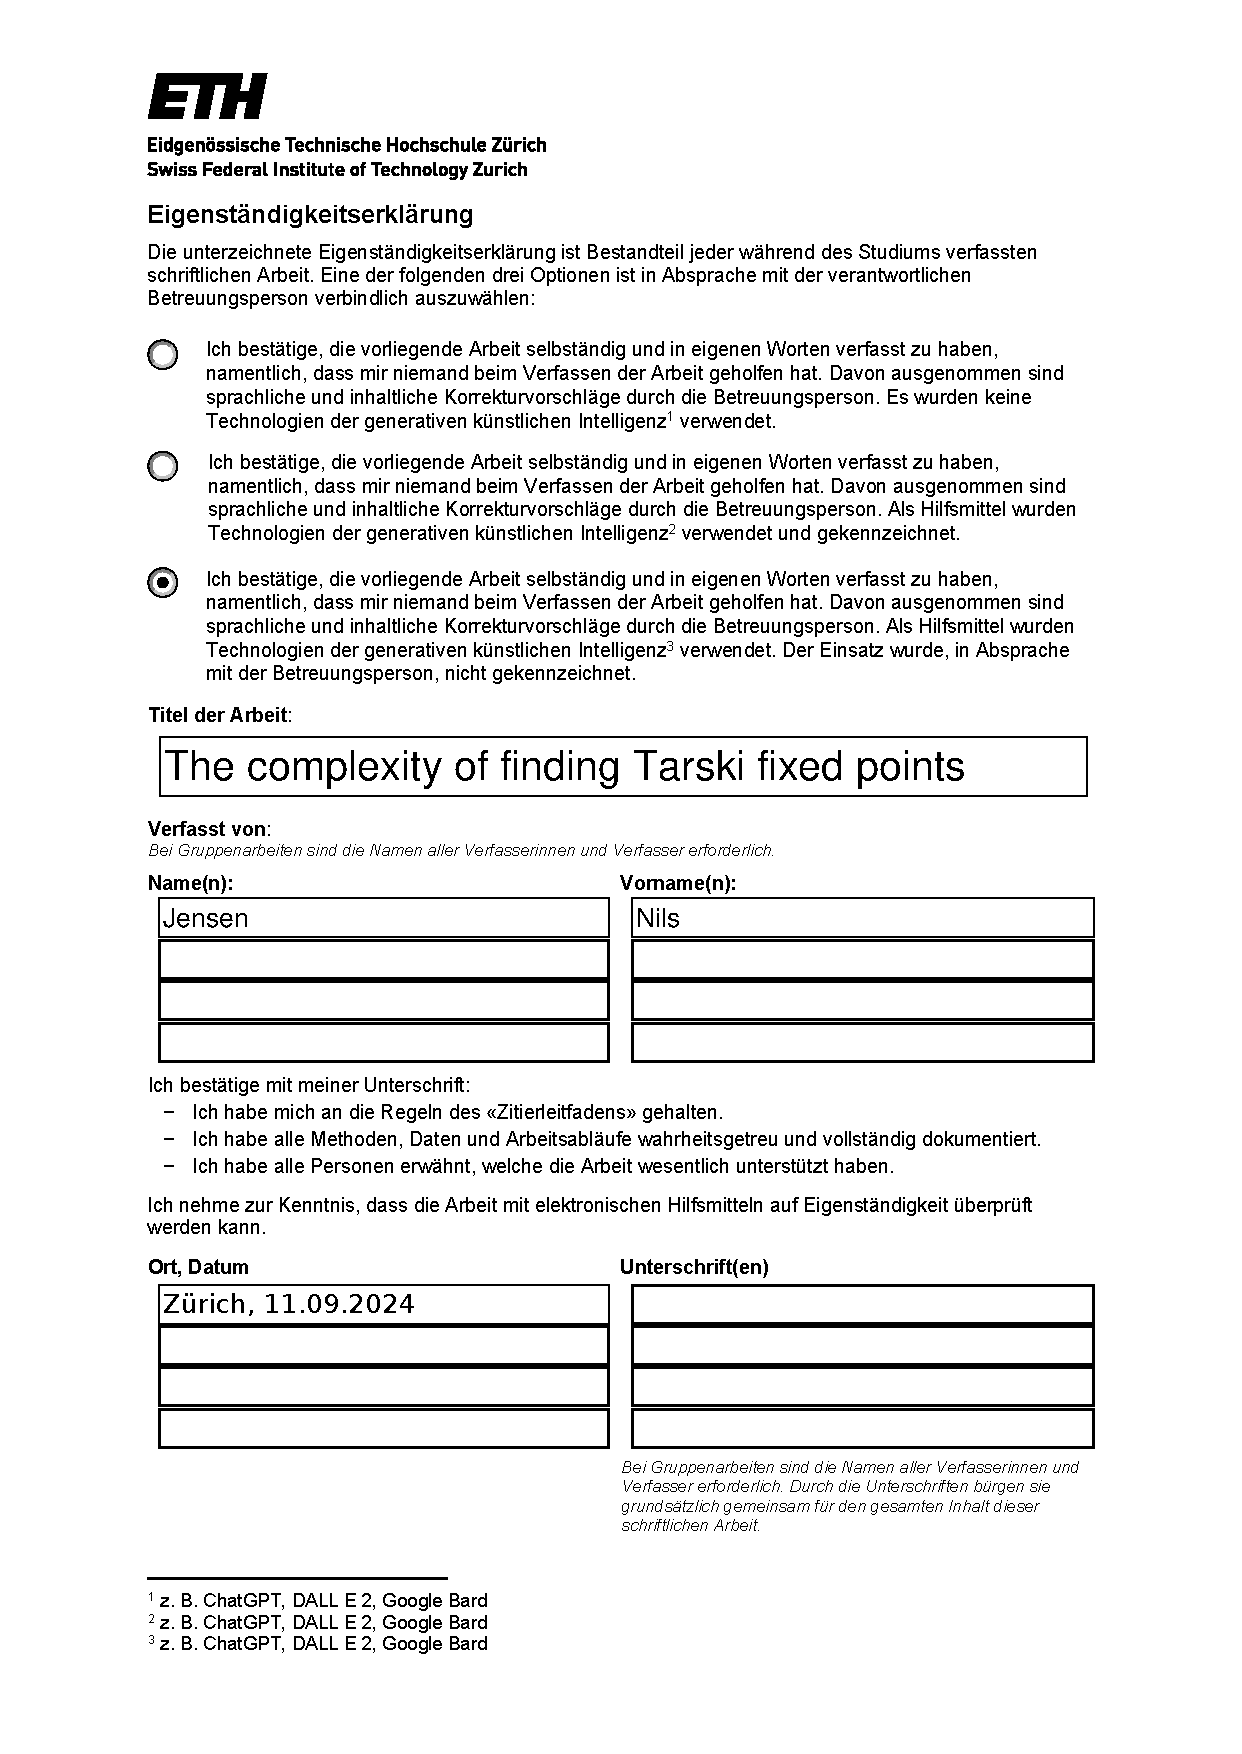
\includepdf{content/Eigenständigkeitserklärung.pdf}

\end{document}
